%%% http://www.dm.unibo.it/studenti/latex/tesi.php

\documentclass[a4paper,12pt]{report}  %inizio documento, solo fronte, tipo report
% \documentclass[a4paper, twoside]{article} %inizio documento, stampato su 2 lati, tipo articolo
\usepackage[italian]{babel} %imposta la lingua a italiano
\usepackage{makeidx} %aggiunge il pakage degli indici
\usepackage{graphicx} %permette di importare i grafici in pdf e immagini
\usepackage{latexsym} %permette di inserire i caratteri speciali
%\usepackage{multirow} %colonne a multiriga
\usepackage[breaklinks]{hyperref} %genera l'indice linkato
%\setcounter{secnumdepth}{-2} % toglie  la numerazione ai capitoli e indice
\usepackage[applemac]{inputenc} %permette la compilazione delle lettere accentate in MacOSX
% \usepackage[utf8]{inputenc} %se non va quello sopra
\usepackage{indentfirst} %serve per avere l'indentazione all'inizio di capitoli, sezioni, etc.
\usepackage{fancyhdr} %serve per impaginare bene la tesi
%\usepackage{showkeys} %serve per mostrare le etichette, 										!!! va tolta per la versione definitiva; 

\pagestyle{plain} %stampa indice a piepagina

\author{Racchetti Luca\\703311}
\title{Tesi}
\date{\today}

\pagestyle{fancy}\addtolength{\headwidth}{20pt}
\renewcommand{\chaptermark}[1]{\markboth{\thechapter.\ #1}{}}
\renewcommand{\sectionmark}[1]{\markright{\thesection \ #1}{}}
\cfoot{}

\rhead[\fancyplain{}{\bfseries\leftmark}]{\fancyplain{}{\bfseries\thepage}}
\lhead[\fancyplain{}{\bfseries\thepage}]{\fancyplain{}{\bfseries\rightmark}}

%\makeindex %genera l'indice

\begin{document} %inizio del documento

%-------------------------------------------------------------------------

\maketitle %genera la prima pagina
\newpage %nuova pagina

%-------------------------------------------------------------------------

\tableofcontents % Indice
%\printindex % stampa l'indice
\newpage %nuova pagina

%-------------------------------------------------------------------------

\chapter{Introduzione} 
	\section{Obiettivo della tesi}

%scopi dello studio
L�obiettivo di questa tesi � quello di:
\begin{itemize}
\item descrivere la filosofia e la pratica che permeano gli Open Data
\item analizzare il processo che ha portato all�attuale situazione legislativa, in particolare la variegata situazione regionale
\item confrontare le piattaforme tecnologiche al momento esistenti
\item spiegare le esigenze implementative del Comune di Vigevano
\item spiegare come questa piattaforma � stata realizzata
\end{itemize}
Infine ha lo scopo di effettuare un�analisi riguardante la reale sostenibilit� da parte del Comune della scelta proposta.

	\newpage
\section{Struttura}
Il secondo capitolo parler� di cosa sono gli Open Data, cercando di darne una definizione che includa le varie sfaccettature di questa nuova pratica e filosofia, del loro ruolo nella societ� e della loro importanza in ambito governativo. Si affronter� l�analisi di chi sono gli attori principali intorno a questo argomento e le loro esigenze. Successivamente si affronter� l�aspetto legale riguardante la materia Open Data, dalla spinta iniziale Americana, fino alle leggi emanate negli ultimi anni nella nostra Penisola. Si far� inoltre un�analisi dell�attuale situazione Italiana per comprendere la differente situazione nelle varie regioni.\\

Nel terzo capitolo si approfondiranno alcune soluzioni tecnologiche, cercando di comprendere la loro architettura, analizzando le caratteristiche offerte e spiegando l�esperienza dell�utente finale.\\

All�interno del quarto capitolo si esaminer� la situazione del Comune di Vigevano, studiando un�adeguata soluzione rispetto all�esigenza di pubblicare le informazioni presenti nelle loro banche dati e alla volont� di integrare la piattaforma che verr� realizzata con quella in uso da Regione Lombardia.\\

Il quinto capitolo descriver� la realizzazione della piattaforma, partendo dall�installazione della piattaforma scelta e proseguendo con la personalizzazione e la creazione delle funzionalit� richieste in fase di progettazione.\\

Nel sesto capitolo sar� fatta una presentazione dell�utilizzo della piattaforma realizzata, cercando di mostrare tutte le sue potenzialit�.\\

Infine nel settimo capitolo sar� fatta un�analisi del lavoro svolto e saranno tratte le dovute conclusioni e ipotizzati gli sviluppi futuri del progetto.
\newpage %nuova pagina

%-------------------------------------------------------------------------

\chapter{Cosa si intende per OpenData} 
	\section{Movimento OpenData}
% Filosofia
%Con il termine Open Data (o dati aperti) si definisce sia la filosofia che la pratica, che prevedono l'esistenza di diverse tipologie di dati accessibili liberamente a tutti, senza restrizioni derivanti da brevetti o copyright, fatta eccezione per le licenze che obbligano a citarne la fonte o al rilascio dei dati modificati con lo stesso tipo di licenza.
\begin{quoting}
I dati aperti, comunemente chiamati con il termine inglese Open Data anche nel contesto italiano, sono alcune tipologie di dati liberamente accessibili a tutti, privi di brevetti o altre forme di controllo che ne limitino la riproduzione e le cui restrizioni di copyright eventualmente si limitano ad obbligare di citare la fonte o al rilascio delle modifiche allo stesso modo. \cite{wiki-datiaperti}
\end{quoting}

Partecipazione, Democrazia, Comunit�, Diritti� sono solo alcune delle parole che vengono associate agli OpenData. Ci� pu� avvenire attraverso il ricorso alle nuove tecnologie dell'informazione e della comunicazione, sulla base delle esperienze positive gi� sperimentate in altri movimenti e comunit� �open�, quali l'\textit{open source}, l'\textit{open access} e l'\textit{open content}. Negli anni la pratica e l'ideologia che caratterizza i dati aperti si � ben consolidata, ma solo recentemente � nata una nuova accezione legata maggiormente al mondo di Internet, che diventa il canale principale di diffusione dei dati stessi, e con essa si identifica il termine �Open Data�. \cite{wiki-datiaperti}.

L'Open Data � una strategia fondamentale della pi� ampia disciplina dell'Open Government, ovvero l'idea in base alla quale la pubblica amministrazione deve essere aperta ai cittadini in termini di trasparenza, di collaborazione e di partecipazione diretta al processo decisionale. Ci� comporta che nell�Open Data non ci sia \textit{e-participation} (partecipazione in processi di governo e di governance), e che i dati siano messi a disposizione dalla Pubblica Amministrazione in sola lettura da parte degli utenti, i quali li utilizzano in base alle loro esigenze:
\begin{itemize}
\item \textbf{Cittadini}: per misurare le performance e la trasparenza della Pubblica Amministrazione (es. dati di bilancio), o per informazione (es. orari mezzi pubblici, sportelli sanitari, ...).
\item \textbf{Giornalisiti}: per cercare informazioni legati a interessi particolari (es. lugli della citt� statisticamente con maggior criminalit�).
\item \textbf{Imprese}: principalmente per analisi di mercato (es. esercizi sul territorio interessati a un prodotto) o per produzione di software che sfrutta l�informazione presente nei dati.
\item \textbf{Pubblica amministrazione}: per migliorare le scelte decisionali (es. un tasso di malattia anomalo pu� essere correlato alla presenza di sostanze tossiche).
\end{itemize}

I dati del governo sono considerati aperti se sono resi pubblici in modo da rispettare gli \textbf{8 principi dell�Open Governament Data}:
\begin{enumerate}
\item \textbf{Completi}: Tutti i dati pubblici sono resi disponibili. Sono dati che non sono soggetti a limitazioni di privacy, di sicurezza o limitazioni di privilegio.
\item \textbf{Primari}: I dati vengono raccolti alla fonte, con il pi� alto possibile livello di �gnaularit��, non in forme aggregate o modificate.
\item \textbf{Tempestivi}: Dati sono resi disponibili in tempi necessari a preservarne il valore e devono essere mantenuti aggiornati.
\item \textbf{Accessibili}: I dati sono disponibili al maggior numero di utenti per i pi� vari scopi.
\item \textbf{Processabili}: I dati vengono adeguatamente strutturati per consentire l'elaborazione automatizzata.
\item \textbf{Non discriminatori}: I dati sono disponibili a chiunque, senza necessit� di registrazione.
\item \textbf{Non proprietari}: I dati sono disponibili in un formato su cui nessun ente ha l�esclusivo controllo.
\item \textbf{Liberi da licenza}:  I dati non sono soggetti a diritti d'autore, brevetti, marchi o segreto commerciale. Possono essere ammesse ragionevoli restrizioni di privacy, sicurezza e privilegio.
\end{enumerate}
In aggiunta agli 8 principi � inoltre importante rendere i dati:
\begin{itemize}
\item \textbf{Riutilizzabili}: Gli utenti devono essere messi in condizione di riutilizzare e integrare i dati, in modo da creare nuove risorse, applicazioni, programmi e servizi di pubblica utilit�.
\item \textbf{Ricercabili}: Facilmente identificabili in rete e facilmente indicizzabili dai motori di ricerca.
\item \textbf{Permanenti}: Le caratteristiche sopra descritte devono caratterizzare i dati nel corso della loro intera vita sul Web.
\end{itemize}

I dati che son stati resi disponibili sono quindi di diverso formato e posso riguardare statistiche o censimenti, dati sensibili accorpati, dati georeferenziati o materiale multimediale.

% scala 5 stelle
\subsection{Scala 5 stelle}
Tim Berners Lee in un suo testo del 2006, successivamente integrato nel 2010 \cite{BernersLee-LinkedData}, per incoraggiare i governi ed altri enti pubblici a rilasciare i dati in formato aperto, introdusse il concetto di \textbf{Dati a 5 stelle}. I concetti trattati nel articolo sono il \textit{Semantic Web} e i \textit{Linked Open Data}, ovvero un particolare tipo di dato strutturato semanticamente che viene pubblicato in rete con licenze di consultazione e d�uso poco restrittive (quali le licenze Creative Commons o le licenze nazionali) e che viene classificato secondo la scala a 5 stelle.\\

\begin{figure}[htbp]
   \centering
   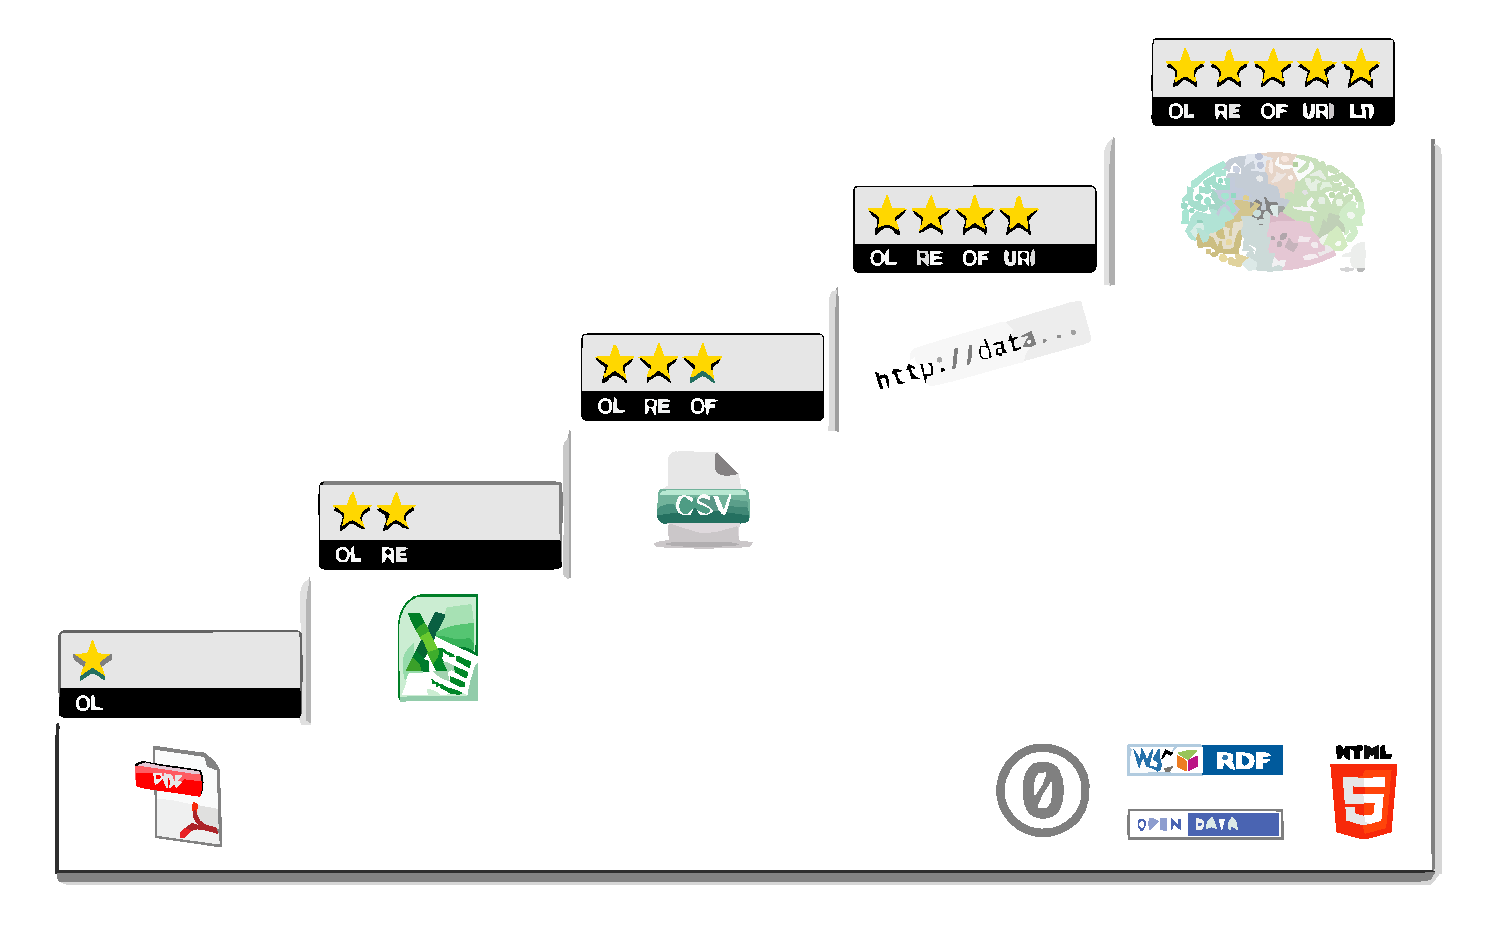
\includegraphics[scale=1.80]{img/5star-steps}
   \caption{Scala a 5 stelle}
   \label{fig:5star-steps}
\end{figure}

La scala a 5 stelle (fig. \ref{fig:5star-steps}) vuole misurare quanto i dati siano aperti e accessibili, assegnando le stelle secondo i seguenti criteri:

%\begin{table}[htbp]
\begin{center}
\begin{tabularx}{\textwidth}{r X}
no star & \textbf{Web data} (in qualsiasi formato) senza nessuna licenza open\\
\ding{72} & Il dato � disponibile sul Web (in qualsiasi formato) con una \textbf{licenza aperta}\\
\ding{72} \ding{72} & Il dato � disponibile in un \textbf{rformato strutturato} (ad esempio un Excel invece della scansione di una tabella) in modo che possa essere iutilizzato\\
\ding{72} \ding{72} \ding{72} & Il dato � in un \textbf{formato non proprietario} (ad esempio un CSV invece di un Excel)\\
\ding{72} \ding{72} \ding{72} \ding{72} & Il dato utilizza gli \textbf{URI} per identificare gli oggetti, in modo che le persone possano far riferimento alle sue risorse e fare uso di RDF\\
\ding{72} \ding{72} \ding{72} \ding{72} \ding{72} & Il \textbf{dato} � \textbf{collegato} ad altri dati per fornire un contesto\\
\end{tabularx}
\end{center}
%\end{table} 

% Obama, ...
\subsection{Open Data in ambito governativo}
Una grossa spinta all'affermazione del movimento Open Data in ambito governativo � stata data dal presidente degli Stati Uniti d'America \textbf{Barack Obama} con la promulgazione di una Direttiva sull'Open government nel dicembre 2009 \cite{Direttiva-OpenGovernament}:

\begin{quoting}
Fin dove possibile e sottostando alle sole restrizioni valide, le agenzie devono pubblicare le informazioni on line utilizzando un formato aperto (open) che possa cio� essere recuperato, soggetto ad azioni di download, indicizzato e ricercato attraverso le applicazioni di ricerca web pi� comunemente utilizzate. Per formato open si intende un formato indipendente rispetto alla piattaforma, leggibile dall�elaboratore e reso disponibile al pubblico senza che sia impedito il riuso dell�informazione veicolata.
\end{quoting}

Alla direttiva � stato dato seguito con la pubblicazione sul sito web \url{Data.gov} di molti dati in formato aperto. Il portale ha infatti lo scopo di raccogliere tutte le informazioni rese disponibili dagli enti statunitensi. \cite{wiki-datiaperti}
Nel maggio 2013 Barack Obama ha firmato un nuovo ordine esecutivo \cite{WhiteHouse-OpenData} che obbliga tutte le agenzie governative ad adottare dati in formato aperto compatibili anche con le future infrastrutture informatiche che verranno adottate negli USA. Le pubbliche amministrazioni dovranno assicurarsi, dove � legalmente consentito, che i dati vengano rilasciati in modo tale da risultare facilmente accessibili e utilizzabili.\\

% Italia
\subsection{Open Data in Italia}
\textbf{In Italia} la spinta iniziale � stata data tra il 2007 e il 2010 dalla volont� di alcune amministrazioni locali che han voluto partecipare al progetto \href{http://www.openstreetmap.org/}{OpenStreetMap}, il quale crea e fornisce dati cartografici, come ad esempio mappe stradali, libere e gratuite a chiunque ne abbia bisogno.
I comuni coinvolti, insieme a dei volontari, hanno condiviso i dati dei propri stradari sotto licenza aperta.

Nel giugno 2010 Renato Brunetta, l'allora Ministro per la pubblica amministrazione e l'innovazione, dichiar� in un intervista l'intenzione di realizzare un portale italiano dell�Open data seguendo il modello dei datagov anglosassoni entro la fine dell'anno. Il 18 Ottobre 2011 il portale \url{dati.gov.it} � stato messo on line.

Nel maggio 2010 la regione Piemonte ha realizzato il proprio portale regionale \url{dati.piemonte.it}. Il sito � ancor oggi una delle esperienze nazionali con la miglior riuscita.
Nel 2011 la regione Emilia-Romagna ha seguito l'esempio piemontese.

A partire da settembre 2011 il Comune di Firenze, grazie anche alla spianta del suo Sindaco Matteo Renzi, ha realizzato il proprio portale \url{opendata.comune.fi.it} rilasciando un dataset al giorno nella fase iniziale. Inoltre Firenze � stato il primo comune a testare OpenBilancio, una visualizzazione dei dati che vuole essere comprensibile da tutti.

Nel marzo 2012 � stata rilasciata la seconda versione della licenza progettata per i dati delle Pubbliche Amministrazioni: Italian Open Data License, indicata come IODL v2.0 \cite{IODL2.0}, priva del vincolo "condividi-allo-stesso-modo" e con la sola richiesta di attribuzione della fonte per il riutilizzo dei dati. \cite{wiki-datiaperti}
	\section{Impianto Normativo}
%http://www.slideshare.net/ernestobelisario/open-data-i-nuovi-obblighi-normativi

Il percorso che ha portato all�attuale normativa in ambito Open Data � lungo e intreccia le sue radici con i concetti di \textit{libert� di informazione} e \textit{trasparenza della pubblica amministrazione} ed ha interessato i governi di differenti nazioni.

\begin{itemize}
\item 4 luglio 1966, viene emanato negli USA il \textbf{Freedom of Information Act} (FOIA) \cite{foia}, �atto per la libert� di informazione�, una legge sulla libert� di informazione, che impone alle pubbliche amministrazioni una serie di regole per permettere a chiunque di sapere come opera il Governo federale.
Il FOIA ha aperto a giornalisti e studiosi l'accesso agli archivi di Stato statunitensi, a molti documenti riservati e coperti da segreto di Stato, di carattere storico o di attualit�. Il provvedimento � stato un punto importante per garantire la trasparenza della pubblica amministrazione nei confronti del cittadino, il diritto di cronaca e la libert� di stampa dei giornalisti.

\item 24 novembre 2000, vengono pubblicate nella Gazzetta Ufficiale le \textbf{Disposizioni per la delegificazione di norme e per la semplificazione di procedimenti amministrativi} (legge 340/2000) \cite{legge340/2000}
\begin{quoting}
Le pubbliche amministrazioni di cui all'articolo 1, comma 2, del decreto legislativo n. 29 del 1993 hanno accesso gratuito ai dati contenuti in pubblici registri, elenchi, atti o documenti da chiunque conoscibili.
\cite{legge340/2000}
\end{quoting}

%Data Quality Act � USA � 2001 (quality, objectivity, utility, and integrity of information)
	%https://en.wikipedia.org/wiki/Data_Quality_Act
	%http://rationalwiki.org/wiki/Data_Quality_Act
	%http://www.gpo.gov/fdsys/pkg/PLAW-106publ554/html/PLAW-106publ554.htm

\item 17 novembre 2003, viene approvata dal Parlamento Europeo e dal Consiglio la \textbf{Direttiva relativa al riutilizzo dell�informazione del settore pubblico} (Direttiva PSI) \cite{direttiva-PSI} che incoraggia gli enti pubblici degli stati membri a massimizzare il potenziale dell'informazione rendendo disponibili e favorendo il riuso dei documenti, attraverso indici on line e licenze standard.

\item 7 marzo 2005, viene approvato il decreto legislativo \textbf{Codice dell'amministrazione digitale} (C.A.D.) \cite{cad}.

\item 24 gennaio 2006, l�attuazione italiana della direttiva europea avviene con il \textbf{Decreto legislativo 24 gennaio 2006 relativo al riutilizzo di documenti nel settore pubblico} \cite{decreto-legislativo2006}. Il provvedimento � stato predisposto dal Ministro per le Politiche comunitarie e da quello per l'innovazione e le tecnologie, in accordo con i dicasteri degli Affari Esteri, Giustizia, Economia e Finanze, Funzione pubblica.
Esso definisce che il titolare del dato predisponga le licenze standard per il riutilizzo e le renda disponibili, ove possibile in forma elettronica, sui propri siti istituzionali.
Gli Enti pubblici possono richiedere un compenso in denaro: in questo caso hanno l'obbligo di fissare e pubblicare le tariffe e le relative modalit� di versamento da corrispondere a fronte delle attivit�, individuandole sulla base dei costi effettivi sostenuti dalle Amministrazioni e aggiornato ogni due anni; questo compenso comprende i costi di raccolta, di produzione, di riproduzione e diffusione dei dati, maggiorati nel caso di riutilizzo per fini commerciali.
� fatto divieto di esclusivit� sull�utilizzo dei dati.

\item 12 giugno 2008, il il Garante per la Protezione dei Dati Personali, in corrispondenza dell�avvio dell�Operazione Trasparenza, ha sottolineato la necessit� di predisporre \textit{�idonei accorgimenti volti a consentire forme proporzionate di consultabilit� dei dati, prevedendo in particolare elenchi relativi a singole amministrazioni, consultabili distintamente (anche sulla base di eventuali link a siti web delle amministrazioni medesime), senza che per gli utenti sia possibile modificarli agevolmente o reperire direttamente dati mediante motori di ricerca�} \cite{nota-12giugno}.

\item 31 ottobre 2009, viene pubblicato in Gazzetta Ufficiale il Decreto legislativo n.150/2009, Attuazione della legge 4 marzo 2009, n. 15, in materia di \textbf{ottimizzazione della produttivit� del lavoro pubblico e di efficienza e trasparenza delle pubbliche amministrazioni} (legge Brunetta) \cite{legge-Brunetta}. Il Decreto indica le linee guida rispetto alle quali articolare il riordino della pubblica amministrazione nella direzione della produttivit�, dell�efficienza e della trasparenza. Le direttrici individuate sono in particolare: il merito, le nuove norme sull�ordinamento del lavoro pubblico, il sistema sanzionatorio e disciplinare e, per quanto riguarda le performance, il ciclo di gestione, la trasparenza e rendicontazione, la misurazione e valutazione.
%Le direttrici individuate sono in particolare: il ciclo di gestione delle performance, la trasparenza e rendicontazione della perfomance, la misurazione e valutazione della perfomance, il merito, le nuove norme sull�ordinamento del lavoro pubblico ed il sistema sanzionatorio e disciplinare.

\item 20 ottobre 2011, viene pubblicato dal Ministero per la Pubblica Amministrazione e l'Innovazione il \textbf{Vademecum sull'OpenData}\cite{vademecum-OD}

\item 22 giugno 2012, viene approvato il Decreto Legge \textbf{Misure urgenti per la crescita del Paese} (Decreto Sviluppo) \cite{decreto-sviluppo}.
\begin{quoting}
Art. 18
\begin{enumerate}
\item La concessione delle sovvenzioni, contributi, sussidi ed ausili
finanziari alle imprese e l'attribuzione dei corrispettivi e dei
compensi a persone, professionisti, imprese ed enti privati e
comunque di vantaggi economici di  qualunque  genere [...] ad enti pubblici e
privati, sono soggetti alla pubblicit� sulla rete internet, ai sensi
del presente articolo e secondo il principio di accessibilit� totale [...]
\item Nei casi di cui al comma 1 ed in deroga ad ogni diversa
disposizione di legge o regolamento, nel sito internet dell'ente
obbligato sono indicati:
\begin{enumerate}
\item il nome dell'impresa o altro soggetto
beneficiario ed i suoi dati fiscali;
\item l'importo;
\item la norma o il
titolo a base dell'attribuzione;
\item l'ufficio e il funzionario o
dirigente responsabile del relativo procedimento amministrativo;
\item la modalit� seguita per l'individuazione del beneficiario;
\item il link al progetto selezionato, al curriculum del soggetto incaricato,
nonch� al contratto e capitolato della prestazione, fornitura o
servizio.
\end{enumerate}
\item Le informazioni [...] sono riportate, con link \textbf{ben
visibile} nella homepage del sito, nell'ambito dei dati della sezione
�Trasparenza, valutazione e merito� [...], \textbf{che devono essere resi di facile
consultazione, accessibili ai motori di ricerca ed in formato
tabellare aperto che ne consente l'esportazione}, il trattamento e il
riuso [...]
\item[5.] A decorrere dal 1� gennaio 2013, per le concessioni di vantaggi
economici  successivi  all'entrata  in  vigore  del  presente
decreto-legge, la pubblicazione ai sensi del presente \textbf{articolo
costituisce condizione legale di efficacia del titolo} legittimante
delle concessioni ed attribuzioni di importo complessivo \textbf{superiore a
mille euro nel corso dell'anno solare previste dal comma 1}, e la sua
eventuale omissione o incompletezza � rilevata d'ufficio dagli
organi dirigenziali e di controllo, \textbf{sotto la propria  diretta
responsabilit� amministrativa,  patrimoniale  e  contabile}  per
l'indebita concessione o attribuzione del beneficio economico. \textbf{La
mancata, incompleta o ritardata pubblicazione � altres� rilevabile
dal destinatario della prevista concessione o attribuzione e da
chiunque altro abbia interesse, anche ai fini} del risarcimento del
danno da  ritardo  da  parte  dell'amministrazione, [...]
\item[7.] Dall'attuazione del presente articolo \textbf{non derivano nuovi o
maggiori oneri a carico della finanza pubblica} e alle attivit�
previste \textbf{si far� fronte con le risorse umane, finanziarie e
strumentali disponibili a legislazione vigente}.
\cite{decreto-sviluppo}
\end{enumerate}
\end{quoting}
Con l�entrata in vigore di questo Decreto Legge inizia a prendere vita �Dentro il bilancio�, un progetto che amplia quello che precedentemente era \textit{OpenFatture}.

\item 18 ottobre 2012, vengono approvate le �Ulteriori misure urgenti per la crescita del Paese� \cite{ulteriori-misure-urgenti} che modificano l�articolo 52 del \textbf{Codice dell�Amministrazione Digitale} (C.A.D.) \cite{cad}. In forza di questa modifica, gli Open Data sono diventati un �obbligo di legge�, nel rispetto della privacy e delle normative a tutela del segreto statistico, brevetti, diritto d�autore, �
\begin{quoting}
L'accesso telematico a dati, documenti e
procedimenti e il riutilizzo dei dati e documenti e' disciplinato dai
soggetti di cui all'articolo 2, comma 2, secondo le disposizioni del
presente codice e nel rispetto della normativa vigente. \textbf{Entro 120
giorni dall'entrata in vigore del presente  decreto-legge, le
pubbliche amministrazioni  pubblicano}  nel  proprio  sito  web,
all'interno della sezione �Trasparenza, valutazione e merito� i
regolamenti che disciplinano l'esercizio della facolt� di accesso
telematico e il riutilizzo, compreso \textbf{il catalogo dei dati e dei
metadati in loro possesso}. 
\cite{ulteriori-misure-urgenti}
\end{quoting}
Le Pubbliche Amministrazioni devono promuovere �progetti di elaborazione e di diffusione dei dati pubblici di cui sono titolari�, nonch� assicurarne la pubblicazione �in formati aperti�, al fine di �valorizzare e rendere fruibili� i dati stessi.
Inoltre viene specificato che a partire dal 19 marzo 2013 tutti i dati e documenti che le pubbliche amministrazioni pubblicano con qualsiasi modalit�, senza l�espressa adozione di una licenza d�uso, si intendono rilasciati come dati aperti (open data by default).

\item 6 novembre 2012, vengono approvate le \textbf{Disposizioni per la prevenzione e la repressione della corruzione e dell'illegalit� nella pubblica amministrazione} (legge anticorruzione) \cite{anti-corruzione}.
% http://saperi.forumpa.it/story/69856/trasparenza-e-anticorruzione-ma-non-chiamatelo-foia

\item 14 marzo 2013, entra in vigore il Decreto Legislativo \textbf{Riordino della disciplina riguardante gli obblighi di pubblicit�, trasparenza e diffusione di informazioni da parte delle pubbliche amministrazioni} \cite{riordino-disciplina} con il quale la l�Amministrazione comunale provvede all�adeguamento delle pagine dei propri siti web.

\item 26 giungo 2013, � stata pubblica la nuova direttiva del parlamento e del consiglio europeo relativa al riutilizzo dell�informazione del settore pubblico \cite{Direttiva-Europea-PSI}: l'open data si estende a biblioteche, archivi e musei. Apertura diventa in pratica sinonimo di riusabilit�.

\end{itemize}


\subsection{Leggi Regionali}

Diverse amministrazioni regionali hanno compreso il valore e l�importanza dell�Open Data e hanno quindi deciso di dotarsi di una Legge in materia \cite{agenzia-regioni}.
Al memento tale processo � ancora in fase evolutiva e la situazione � piuttosto variegata nella nostra penisola (fig. \ref{fig:leggi-regionali}).


\begin{figure}[htbp]
   \centering
   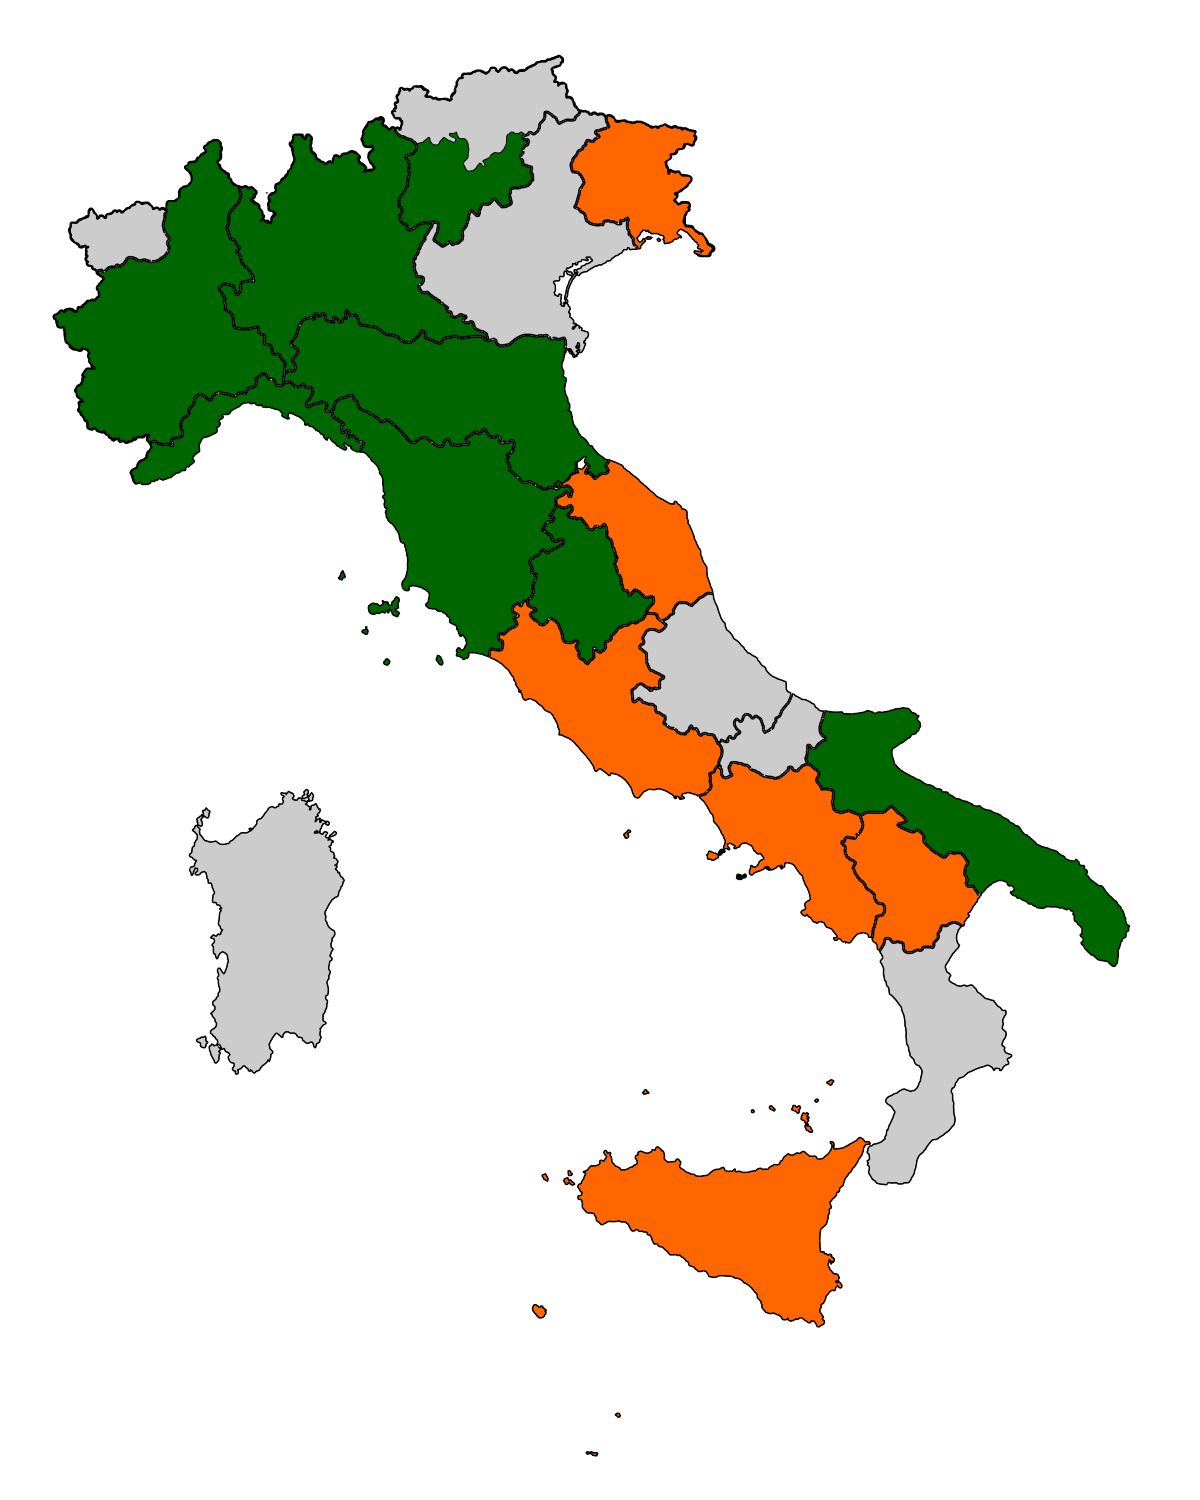
\includegraphics[scale=0.35]{img/Italia-OpenData} % requires the graphicx package
   \caption{Situazione normativa nelle Regioni italiane su Open Data:\protect\newline \textbf{Verde}:  legge approvata.\protect\newline \textbf{Arancione}: disegno o proposta di legge in discussione.}
   \label{fig:leggi-regionali}
\end{figure}


\begin{itemize}
\item \textbf{Lombardia}: Nell�Agenda Digitale di Lombardia per il periodo 2012-2015 (DGR 2585/2011) � inclusa l�Area Prioritaria d�Intervento �Patrimonio Informativo Pubblico�, (paragrafo 2.4).
Con la delibera 2094/2012 si approvano i �Criteri generali per l�open data�.
Con La LR N. 7/2012 - art. 52 Accessibilit� e valorizzazione del patrimonio informativo pubblico - la Giunta regionale, adotta determinazioni in ordine alla definizione delle basi di dati regionali da rendere disponibili a cittadini ed imprese in formato aperto, nonch� le modalit� di fornitura, senza oneri per finanza regionale, dei dati rilevati nell�esercizio delle attivit� da parte di concessionari di servizi pubblici.
Il DG 6115/2012 definisce il Modello di Governance, stabilendo ruoli e modalit� d�intervento per rendere disponibili i dati del patrimonio informativo regionale come Open Data ed il metodo con cui sono pianificati gli interventi, e il DGR n. 4324/2012 costituisce le linee guida per gli EELL che ripropongono, principalmente ai Comuni Lombardia, il modello organizzativo e le scelte operative adottate da Regione per la gestione degli Opendata.

\item \textbf{Umbria}: Nell�Agenda Digitale dell�Umbria (DGR 397/2012) � inclusa tra le linee prioritarie d�azione quella dedicata agli open data.
Nella legge regionale n.8/2011 sulla semplificazione e sullo sviluppo dell�Amministrazione digitale l�art.15 prevede la promozione dei dati pubblici aperti.
Con D.G.R. 1551/2012 � stato approvato il Disciplinare dei criteri generali per l�open data in Umbria, vincolante per l�Amministrazione regionale e di riferimento per gli enti del territorio (che sono invitati a pubblicare i loro dati nel repertorio regionale).

\item \textbf{Toscana}: Il Programma regionale per la promozione e lo sviluppo dell�amministrazione elettronica e della societ� dell'informazione e della conoscenza (DGR 104/2012), si pone come agenda digitale regionale prevede un�azione specifica relativa all�apertura dei dati.
La successiva evoluzione normativa in materia di amministrazione digitale consta di tre Leggi Regionali (LR 1/2004, LR 40/2009 e LR 54/2009).
La LR 40/2009 (e s.m.i.) in riferimento alla trasparenza e all�attivit� amministrativa, ambito pi� ampio e precedente rispetto allo specifico degli open data, tratta il diritto di accesso.
La LR 54/2009 pone riferimenti importanti alla politica di open data, tra questi il principio per cui lo sviluppo dell�amministrazione digitale deve avvenire con il coinvolgimento degli enti del territorio.
L�attuazione degli open data � definita con DGR 23/2013, con cui l�apertura dei dati si pone come necessario passaggio culturale ed elemento per arrivare anche all�apertura dei servizi.

\item \textbf{Emilia Romagna}: Con DGR 52/2011 sono state approvate le nuove Linee Guida al Piano Telematico regionale 2011-2013 (PiTER), documento che rappresenta l�Agenda Digitale regionale.
La Giunta della Regione Emilia-Romagna ha successivamente approvato con delibera 1587/201 il Programma Operativo 2011 del PiTER con il quale � stata data concretezza agli obiettivi strategici enunciati nelle Linee Guida, consolidando le azioni intraprese e future in un progetto operativo sottoposto a monitoraggio e valutazione.
Con successiva DGR 2080/2012, Emilia approva le �Linee guida relative al riutilizzo e messa a disposizione in Open Data dei dati pubblici dell�Amministrazione Regionale con i quali condivide il valore e la funzione attribuiti dall'Unione Europea alle informazioni pubbliche, e la consapevolezza delle conseguenze positive a livello di trasparenza e di partecipazione attiva dei cittadini alle attivit� e alla vita delle Pubbliche Amministrazioni, a seguito della diffusione di tali informazioni.

\item \textbf{Piemonte}: � un esempio significativo con il processo che parte con l�emissione di linee guida nel 2009 (DGR 11679/2009) che definiscono i processi di riuso, e un aggiornamento delle stesse nel 2010 (DGR 1109/2010). Segue l�adozione della Legge Regionale in materia (LR 24/2011) e relativo regolamento attuativo con la quale Regione si vincola ad assicurare la disponibilit�, la gestione, l'accesso, la trasmissione, la conservazione e la fruibilit� dei dati in modalit� digitale.
Detto regolamento si distingue rispetto ad altri casi perch� stabilisce la possibilit� per l�utente esterno, di qualunque tipologia (privato cittadino, ente privato etc.), di presentare formale richiesta per il rilascio in modalit� open di un determinato dataset di suo interesse, e delinea il processo interno dell�Ente per l�adempimento della richiesta. L�utente che non vedesse accolta la propria richiesta senza giustificato motivo ha inoltre la possibilit� di sporgere formale reclamo.

\item \textbf{Puglia}: La LR 20/2012 �Norme sul software libero, accessibilit� di dati e documenti e hardware documentato� tratta i temi dell�Open Data specificatamente all�art. 6 �Riutilizzo dei documenti e dei dati pubblici�.
Le prime Linee di indirizzo in materia di OD sono state oggetto della DGR 2183/2012.

\item \textbf{Provincia Autonoma di Trento}: Il percorso normativo ha inizio con l�emissione delle DGR 1510/2010 e DGR 1510/2011, delibere inerenti alla definizione di una Strategia di Legislatura in materia di innovazione e servizi ICT. Con la prima si introducono gli Open Government Data tra le infrastrutture abilitanti l�innovazione quale condizione necessaria per lo sviluppo dell�innovazione nei servizi; nella seconda si esplicita il l�obiettivo di valorizzare il patrimonio informativo della PA al fine di aumentare la trasparenza, semplificare e rendere pi� efficiente il sistema pubblico e fornire risorse informative ai settori produttivi. Segue l�adozione della LP 16/2012 sulla promozione della societ� dell�informazione e amministrazione digitale.
Con DGR 2858/2012 sono approvate le linee guida per la diffusione e riutilizzo di dei dati pubblici.

\item \textbf{Liguria}: La Regione ha fatto proprie le politiche di pubblicazione dei dati pubblici regionali, in linea con il principio di trasparenza, in considerazione del grande valore attribuito all�economia immateriale e alla luce delle prescrizioni della legge regionale 42/06 �Istituzione del Sistema informativo integrato regionale per lo sviluppo della Societ� dell'informazione in Liguria".

%---

\item \textbf{Regione Lazio} Legge Regionale n. 7/2012 - "Disposizioni in materia di dati aperti e riutilizzo di informazioni e dati pubblici e iniziative connesse�.\\
Proposta di legge n. 200/IX - "Norme in materia di pubblicazione e riutilizzo dei dati e delle informazioni delle pubbliche amministrazioni regionali"

\item \textbf{Regione Basilicata} Proposta di legge - "Disposizioni in materia di accesso, pubblicazione e riutilizzo dei documenti e dei dati pubblici dell'Amministrazione regionale in formato aperto tramite la rete internet"

\item \textbf{Regione Sicilia} Disegno di legge - "Norme in materia di pubblicazione tramite la rete internet e di riutilizzo dei documenti e dei dati della pubblica amministrazione regionale e locale"

\item \textbf{Regione Friuli Venezia Giulia} Legge Regionale n. 9/2011 - "Disciplina del sistema informativo integrato regionale del Friuli Venezia Giulia"

\item \textbf{Regione Campania} Proposta di legge - "Legge sulla trasparenza amministrativa e l'accesso e il riutilizzo dei dati di titolarit� regionale"

\item \textbf{Regione Marche} Proposta di legge n. 256/12 -  �Disposizioni in materia di pubblicazioni e riutilizzo dei dati e delle informazioni dell�amministrazione regionale�


\end{itemize}


%------------------------------
\subsubsection{Regione Lombardia}
La Regione Lombardia ha approvato, con la Delibera di Giunta Regionale 2904 del 11/01/2012 i "Criteri generali per l'open data" \url{http://www.agendadigitale.regione.lombardia.it/shared/ccurl/96/714/dgr\%202904\%20open\%20data.pdf} nei quali delibera di realizzare la piattaforma \url{dati.lombardia.it} sulla quale caricare, in una prima fase, i dati gi� pubblicati sui portali della Regione e sul sistema SIREG. Delibera inoltre di pubblicare dati aggregati di cui la Regione � proprietaria, il tutto con una licenza che concede all'utente la possibilit� di riprodurre, distribuire, trasmettere e adattare liberamente i dati, anche a scopi commerciali, a condizione che venga citata la fonte, la licenza che � stata scelta � la Italian Open Data License v.2.0 (IODL 2.0).\\

\subsubsection{Comune di Vigevano}
Il Comune di Vigevano il 23 maggio 2013 ha deliberato l�\textbf{Adesione alle �Linee guida Open Data per gli enti locali�, di Regione Lombardia e sperimentazione congiunta in materia} \cite{CittaVigevano-GCn104}:
\begin{quoting}
\begin{enumerate}
\item di aderire alle �Linee Guida per gli Enti Locali� facendo propri i relativi allegati e usufruendo per la diffusione dei dati individuati come riutilizzabili del portale \url{dati.lombardia.it};
\item d'impegnarsi, coerentemente con quanto previsto dalle Linee Guida, a licenziare i dati � quale regola generale - con licenza IODL 2.0, optando a favore di altre licenze solo ove ricorrano giustificati motivi; la licenza scelta dovr� comunque consentire il riutilizzo dei dati pubblicati anche per fini di lucro e commerciali, come richiesto dai �Criteri generali per l�Open Data�, Allegato 1 alla DGR 2904 dell�11/1/2012;
\item di avviare una collaborazione \textbf{con Regione Lombardia / Lombardia Informatica} sui temi della interoperabilit� dei Open Data pubblicati in portali diversi tramite l�uso principale di soluzioni Open Source con l�obiettivo, fra gli altri, di consentire un pi� semplice accesso ai dati del futuro portale Open Data del \textbf{Comune di Vigevano} anche attraverso l�accesso dal portare della \textbf{Regione Lombardia}
\cite{CittaVigevano-GCn104}
\end{enumerate}
\end{quoting}
\newpage %nuova pagina

%-------------------------------------------------------------------------

\chapter{Piattaforme Tecnologiche} 
	\section{Socrata (OpenSource)}
% Versione Open Source
Socrata � una piattaforma sviluppata dall'omonimia societ� con sede negli Stati Uniti d'America. Socrata � un servizio "Software as a service".
Dal 10 aprile 2013 � disponibile anche in una versione Community Edition rilasciata come OpenSource al fine di promuovere uno standard intorno ai dati aperti e far crescere la comunit�.

Il Socrata Open Data Server e le componenti che lo compongono sono stati resi disponibili con licenza Apache. 
L�architettura del sistema pu� quindi essere suddivisa in una serie di componenti separate che la compongono come mostrato in figura \ref{fig:socrata-architecture}.

\begin{figure}[htbp]
   \centering
   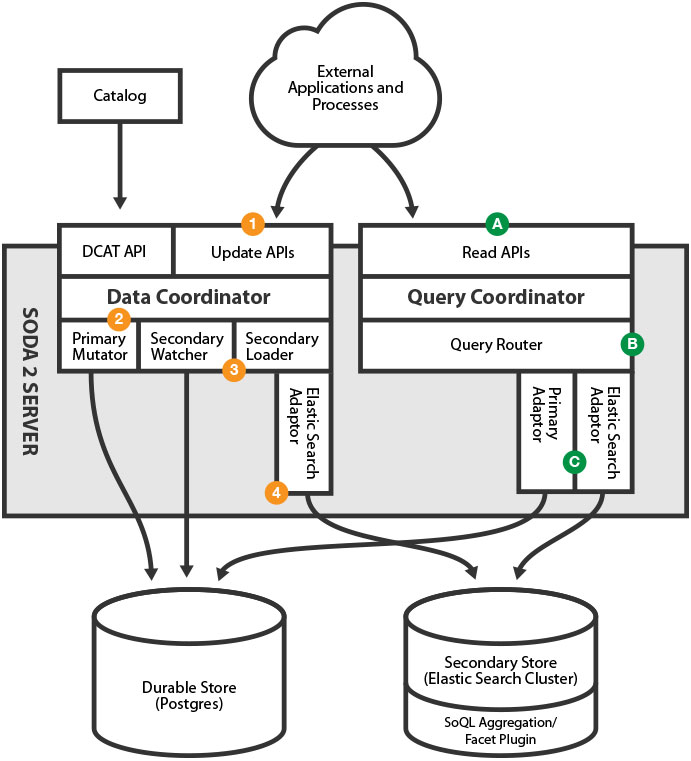
\includegraphics[scale=0.55]{img/socrata-architecture.jpg}
   \caption{Architettura di Socrata}
   \label{fig:socrata-architecture}
\end{figure}

SODA 2 fornisce quindi l�accesso ai dati puri attraverso SoQL (SODA Query Language) e delle semplici API per aggiornarli.
La scrittura avviene quindi attraverso un percorso che prevede il seguente percorso:
\begin{enumerate}
\item[\textcolor{Orange}{\ding{202}}] Un applicazioni o un processo inizia un operazione sul SODA Server.
\item[\textcolor{Orange}{\ding{203}}] La richiesta viene trasformata in una serie di operazioni pi� elementari chiamante �mutations� e vengono passate al Data Coordinator in modo da essere eseguite sul database (Postgres).
\item[\textcolor{Orange}{\ding{204}}] Dopo che il Data Coordinator ha finito, il Secondary Watcher si sveglia e guarda se ci sono cambiamenti nel database che non sono ancora stati sincronizzati.
\item[\textcolor{Orange}{\ding{205}}] L�adattatore per l�archivio secondario (in questo caso Elastic Search) importa i dati dal primario.
Ci� permette in caso di guasti di re-sincronizzare il database.
\end{enumerate}

Mentre la lettura avviene attraverso:
\begin{enumerate}
\item[\textcolor{Green}{\mycirc{\tiny{A}}}] Un applicazione invia una richiesta al server SoQL. Questa viene analizzata come descritto serctitto in soql-reference.
\item[\textcolor{Green}{\mycirc{\tiny{B}}}] Il Query Coordinator determina a quale database inviare la richiesta (in futuro ci portano essere diversi archivi secondari).
\item[\textcolor{Green}{\mycirc{\tiny{C}}}] Il Query Coordinator passa fuori la query all�adattatore appropriato che esegue la query sull�archivio corretto e restituisce l'appropriato payload C-JSON.
\end{enumerate}

Ad oggi sono state rese disponibili con licenza Open Source solo alcune parti:

\begin{itemize}
\item \textbf{soql-reference}, Implementazione di riferimento del linguaggio di interrogazione SoQL.
\item \textbf{socrata-http}, Toolkit per la creazione di servizi HTTP.
\item \textbf{soql-es-adapter}, ElasticSearch Secondary Store per SoQL Data Service.
\item \textbf{socrata-csv}, Un sottile involucro Scalaish intorno ad opencsv.
\item \textbf{socrata-utils}, Classi-Utility utilizzate in tutto il Socrata Open Data Server.
\item \textbf{data-coordinator}, Coordina la distribuzione degli aggiornamenti tra archivi di dati primari e secondari.
\end{itemize}

La Community Edition condivide lo stesso core della versione proprietaria, ma al momento manca completamente il front-end per gestire comodamente i dataset che � invece presente nella versione SaaS.
Secondo la Roadmap intorno all'Agosto 2013 era previsto il rilascio della versione beta finale, compresa della documentazione e degli strumenti che avrebbero permesso di installare e rendere funzionate l'intero Open Data Server.

Socrata offre sia numerose API per gestire i dataset, che strumenti di visualizzazione che mostrano i dati caricati attraverso un sistema di preview tabellare dotato di filtri avanzati, oppure su diverse tipologie di mappe in caso di dati geolocalizzati.
Permette inoltre di esportare i dati in vari formati (CSV, XLS, XLSX, XML, JSON).

In Italia Socrata � stata usata con successo dalla Regione Lombardia con un centinaio di dataset pubblicati.
	\section{CKAN}
CKAN (Comprehensive Knowledge Archive Network) � un potente sistema DMS (Data Management System, ovvero un sistema di gestione dei dati) open source.
Esso ha lo scopo di rendere i dati accessibili permettendo la loro archiviazione e distribuzione attraverso una comoda interfaccia web che ne semplifica la pubblicazione, la condivisione, la ricerca e l'utilizzo.

CKAN offre sia numerose API per gestire i dataset, che strumenti di visualizzazione che ne permettono un rapida anteprima.
La piattaforma supporta molto bene i dati in formato tabellare, siano essi semplici CSV o EXCEL, e la loro visualizzazione pu� essere fatta in semplice tabella, come grafico a punti o su una mappa in caso di dati geolocalizzati.

CKAN � rivolto ai data publishers, come governi, imprese o organizzazioni nazionali/regionali, che vogliono rendere disponibili e facilmente fruibili i propri dati. A ci va aggiunta la possibilit� di integrare facilmente i cataloghi di altri portali sviluppati anch'essi in CKAN.

Il suo codice � mantenuto dalla Open Knowledge Foundation ed � utilizzato come piattaforma per gestire cataloghi pubblici da siti come \url{thedatahub.org}, \url{catalog.data.gov}, \url{data.gov.uk} e \url{PublicData.eu}.

CKAN pu� essere installato gratuitamente su un server di propriet� dello stesso soggetto che intende pubblicare i dati, oppure � possibile acquistare il servizio di hosting dedicato gestito dallo stesso produttore di software (quindi in modalit� SaaS).

CKAN ha iniziato il suo sviluppo nel 2007, ma solo nel maggio 2010 � stata pubblicata la sua prima versione (1.0), alla quale sono seguiti aggiornamenti minori fino alla versione 1.8, che nel maggio 2013 � stata superata dalla nuova versione 2.0. Attualmente � in sviluppo la visione 2.2.

	\section{Sister.it}
\newpage %nuova pagina

%-------------------------------------------------------------------------

\chapter{Progettazione portale OpenData a Vigevano} 
	\section{Descrizione del Comune}
% Storia
La citt� di Vigevano si trova a 30 chilometri da Milano, la fitta vegetazione che cresce ai bordi del Ticino e degli altri canali che attraversano la citt� offre al visitatore magnifici scorci e oasi naturali.

La citt� ha la sua origine come luogo fortificato longobardo dove ora sorge il cortile del castello, successivo � lo sviluppo del borgo esterno, oggi occupato dalla Piazza Ducale.

A partire dal 1198 si trasforma in un libero Comune, mentre nel 1277 la storia delle potenti famiglie milanesi dei Visconti e degli Sforza si lega a quella di Vigevano. Grazie all'opera di Luchino Visconti e di Ludovico Sforza, detto il Moro, tra il XIV e il XV secolo, il borgo di Vigevano inizia la sua trasformazione in residenza estiva: il castello viene adibito a dimora di prestigio, grazie all'opera di artisti come Bramante, e la Piazza Ducale, liberata da case ed edifici, diviene il regale atrio d'ingresso al castello.

Nel 1530 Vigevano ottiene il titolo di citt� con una propria sede vescovile.\\

\textbf{Piazza Ducale}, una delle piazze pi� belle d'Italia, fu ideata e decorata dal Bramante con il concorso di Leonardo da Vinci, che non partecip� direttamente ai lavori, ma lasci� disegni e testimonianze scritte nei codici d'appunti. La piazza funge da ingresso d'onore al Castello. I lavori iniziarono nel 1492 e si conclusero nel 1494. Piazza Ducale rappresenta una delle prime piazze rinascimentali sul modello di ``forum'' romano e uno dei migliori esempi dell'architettura lombarda del XV secolo. Si presenta come un rettangolo di 134 metri di lunghezza e 48 di larghezza, edificato su tre lati. La forma architettonica � opera del vescovo-architetto Juan Caramuel Lobkowitz, che chiuse il quarto lato con la facciata barocca della Chiesa Cattedrale.
Sotto i portici, le botteghe, un tempo occupate dai commercianti di lana e seta, oggi offrono ai visitatori svariate occasioni di svago.\\

\textbf{Il castello} sorge nella parte pi� alta di Vigevano e costituisce una piccola citt� nella citt�, essendo uno dei pi� grandi d'Europa. Anche alla sua realizzazione parteciparono Bramante e Leonardo che contribuirono a dargli il fascino rinascimentale che ancor oggi conserva. Tra il 1492 e il 1494 i lavori furono terminati e le lussuose sale interamente affrescate, in modo da poter ospitare la corte ducale e i loro ospiti, quali il re di Francia Carlo VIII e, pi� avanti, l'imperatore Carlo V.
Con la fine della dinastia sforzesca (1535) il castello pass� agli spagnoli e inizi� un lento declino che lo vide ospitare solo eserciti e trasformarsi in caserma fino al 1960.
Da quella data � iniziato il restauro ed il Castello si sta trasformando in una cittadella dell'arte e della cultura grazie ai suoi musei visitabili - tra cui il curioso e unico in Italia Museo della calzatura - e a un ricco programma di mostre ed eventi musicali nel corso di tutto l�anno.
\cite{ComuneVigevano-CenniStorici}

\subsection{Servizio Informatico Comunale}
% Organizzativo sistemi informativi
Durante la progettazione del portale OpenData per il Comune di Vigevano, il Dipartimento di Informatica Sistemistica e Comunicazione (DISCo) dell'Universit� di Milano Bicoca si � relazionato con il responsabile del Servizio Informatico Comunale (SIC) \href{malto:obaracchi@comune.vigevano.pv.it}{\textbf{Oscar Baracchi}}.\\

Il SIC � la struttura organizzativa cui compete la gestione del sistema informativo dell�Ente (il Comune di Vigevano), attraverso alcune decine di server con supporto ad oltre 350 utenti utilizzatori di apparecchiature informatiche, appositamente configurate per l'accesso alle informazioni presenti nelle banche dati dell�Ente ed alle procedure per l�erogazione di servizi ai cittadini ed alle imprese.

Il Servizio cura la pianificazione, lo sviluppo, il mantenimento, il coordinamento ed il controllo di tutte le iniziative ed attivit� che afferiscono i sistemi informativi comunali, le infrastrutture informatiche, la rete trasmissione dati, la conduzione di progetti nel campo dell�ICT di notevole complessit� tecnologica ed organizzativa.

In particolare il Servizio ha la responsabilit�:
\begin{itemize}
\item della pianificazione strategica e tattica per tutti gli aspetti relativi all�utilizzo dell�ICT (Information \& Communication Technology) nell�Amministrazione Comunale;
\item dello sviluppo di nuove iniziative ed attivit� per il miglioramento del grado di efficienza ed efficacia dell�azione amministrativa tramite l�utilizzo di opportuni sistemi informativi, infrastrutture informatiche e telematiche;
\item del mantenimento in efficienza dei sistemi informativi comunali, delle infrastrutture ed apparecchiature informatiche, di rete trasmissione dati utilizzate nell�Amministrazione comunale;
\item di centro acquisitore per quanto riguarda le forniture di beni e servizi che rientrino nell�ambito dell�ICT;
\item del supporto nella gestione di progetti ed attivit� in cui sia presente una componente informatica o telematica;
\item della consulenza e supporto alle unit� organizzative dell�Amministrazione comunale su aspetti che attengono in qualche misura all�ICT;
\item del supporto nella gestione di progetti ed attivit� di e-government e sovracomunali;
\item del supporto nei rapporti con i fornitori di servizi, tecnologie e soluzioni;
\end{itemize}
    Inoltre sono stati sviluppati e manutenuti in proprio, gi� da anni, con tecnologia web (Java-Jsp) su database MySql ed application server Tomcat/Apache, numerosi applicativi.
\cite{ComuneVigevano-SIC}

	\section{Progettazione piattaforma}

Con delibera 14 del 19/01/2012 il Comune di Vigevano, nell'ambito del Progetto InnoVi, cofinanziato dalla regione, ha adottato, in riuso dal Comune di Milano, la piattaforma \textbf{GIT} \cite{CittaVigevano-GCn104}.

La piattaforma GIT, di propriet� della Pubblica Amministrazione italiana e realizzato attraverso un progetto (GIT �Gestione Intersettoriale del Territorio�) del programma ELISA del Dipartimento Affari Regionali realizzato da Comuni, � stata implementata al fine di integrare, relazionare e rendere interoperabili i dati in possesso di  un ente per il territorio di competenza.
GIT costituisce la dorsale sulla quale i dati possono transitare al fine di acquisire un maggior livello di accuratezza, attendibilit� e completezza.

Pur preservando la peculiarit� di poter rendere disponibili i dati grezzi, rispettando l�indicazione �ROW DATA NOW�, il processo di pubblicazione pu� essere realizzato in modo progressivo attraverso il trattamento dell�informazione per renderla pi� chiara, relazionata e dunque economicamente pi� vantaggiosa per il fruitore finale.

Gli Elementi conoscitivi del territorio sono stati catalogati per la piattaforma in tematismi:

\begin{itemize}
\item         Soggetti che si muovono sul territorio e che agiscono con interazione diretta o intermediata.

\item     Oggetti presenti sul territorio che costituiscono strumenti dell�azione dei Soggetti, Patrimonio economico rappresentativo del valore stesso dei luoghi e contenitori in grado di generare lavoro per la loro conservazione e manutenzione.

\item         Ambiente che caratterizza il territorio amministrato e costituisce un importante riferimento per le regole del vivere civile per la valorizzazione del patrimonio naturale e di manufatti da gestire, valorizzare e preservare.

\item         toponomastica e geolocalizzazione dei luoghi degli oggetti, e delle persone che rappresenta la mappatura e il riferimento per la ricerca, la misurazione e la relazione delle informazioni territoriali di interesse.
\end{itemize}

Attraverso queste �chiavi� di conoscenza primarie del territorio, i dati delle singole fonti vengono assunti come elementi descrittori, analizzati, diagnosticati e  resi disponibili in modo integrato per la consultazione o per l�utilizzo attraverso canali consultazione puntuale, di estrazione e pubblicazione massiva.

La piattaforma GIT � costituita da componenti software realizzati per assicurare determinate funzioni di trattamento delle informazioni, oltre che da servizi di navigazione trasversale fra le fonti e da servizi verticali specialistici, anche cartografici.

Ma sono le funzioni di trattamento delle fonti dati e di orchestrazione, implementate dal componente Controller a poter dare un valore aggiunto al processo di apertura dei dati, si descrivono ora brevemente le peculiarit� e le funzioni principali:

\begin{itemize}
\item   sistema di reperimento e acquisizione dell�informazione attraverso varie modalit� e protocolli. I sistemi operazionali e/o gli utenti possono depositare su repository relazionali / ftp / file system i loro dati  e la piattaforma si preoccuper� di importare tali dati con periodicit� stabilit�. Oppure possono essere implementate e configurate delle sonde applicative che controllano lo stato di variazione aggiornamento di una determinata fonte dati (relazionale e non) al fine di importare le variazioni nel sistema GIT.

\item   Catalogo configurabile e programmabile tramite API di diagnostiche sulle informazioni oggetto di importazione, Le diagnostiche sono uno strumento da asservire al processo di bonifica di un dato per valutarne il grado di qualit� e definire dunque eventuali step successivi. Le diagnostiche sono di due tipi: controllo e confronto; il sistema valuta la qualit� del dato  in termini di obbligatoriet� di attributi informativi, formati e codifiche (controllo) e ne valuta inoltre le anomalie rispetto ad altre fonti informative (confronto). Un esempio di questa seconda tipologia di diagnostica � il �controllo del numero di famiglie in un immobile rispetto al numero di unit� abitative e al numero di contratti di fornitura della rete elettrica o idrica�. Le diagnostiche di confronto, utilizzate in GIT al fine di indagine e ricerca di �anomalie�, pu� essere sfruttata nella generazione di relazioni interne di tipo appunto semantico.

\item   Sistema di correlazione delle fonti dati basato sui tematismi Soggetto, Via, Civico, Oggetto Territoriale e Fabbricato. Attraverso un sistema di metadati vengono caratterizzati gli attributi di un archivio in modo da poter attribuire ad ognuno una categoria e un tipo. Per esempio vengono classificati tutti gli archivi che si riferiscono ad un immobile e all�interno di ogni archivio vengono identificati gli attributi territoriali (via, civico, coordinate catastali ecc.). Attraverso algoritmi standard di ricerca sql, attraverso l�utilizzo di algoritmi dinamici per la ricerca delle similarit� e di algoritmy fuzzy ogni record di una fonte informativa viene correlato ad altri di altre fonti con un determinato grado di attendibilit�. Queste correlazioni sono alla base di alcuni algoritmi diagnostici per la ricerca dell�evasione fiscale e alla base del sistema di navigazione dinamico GIT.

\item   Trattamento di dati cartografici, anche all�interno della correlazione delle informazioni, oltre che negli algoritmi diagnostici al fine di collegare il maggior numero di informazioni alfanumeriche ad un riferimento geografico. La presenza in GIT del catasto terreni / fabbricati, della toponomastica e di altre fonti dati (concessioni, tributi) contenenti riferimenti geografici certi ha permesso di implementare algoritmi deduttivi che attribuiscono gli attributi di localizzazione a fonti dati altrimenti sprovviste di questa informazione. Questo permette potenzialmente di visualizzare graficamente all�interno di un WebGIS quasi tutte le fonti dati. 

\item   Presenza di un catalogo dei dati cartografici dinamico in grado di dare la possibilit� di ingessare e tipizzare qualsiasi fonte dati spaziale.
\end{itemize}


Il sistema GIT � quindi un ricco contenitore di informazioni alfanumeriche e grafiche correlate, periodicamente aggiornate, e che, per questo, � un candidato naturale ad alimentare dei dataset di dati da rendere disponibili con licenze open, opportunamente filtrati ed aggregati allo scopo di tutelare la privacy.


Di conseguenza si vuole realizzare una piattaforma che permetta di integrare le informazioni presenti sulla piattaforma GIT con il portale Open Data che verr� realizzato.
Per fare ci� sono percorribili (come mostrato in figura \ref{fig:git-ckan}) tre strade distinte:

\begin{figure}[htbp]
   \centering
   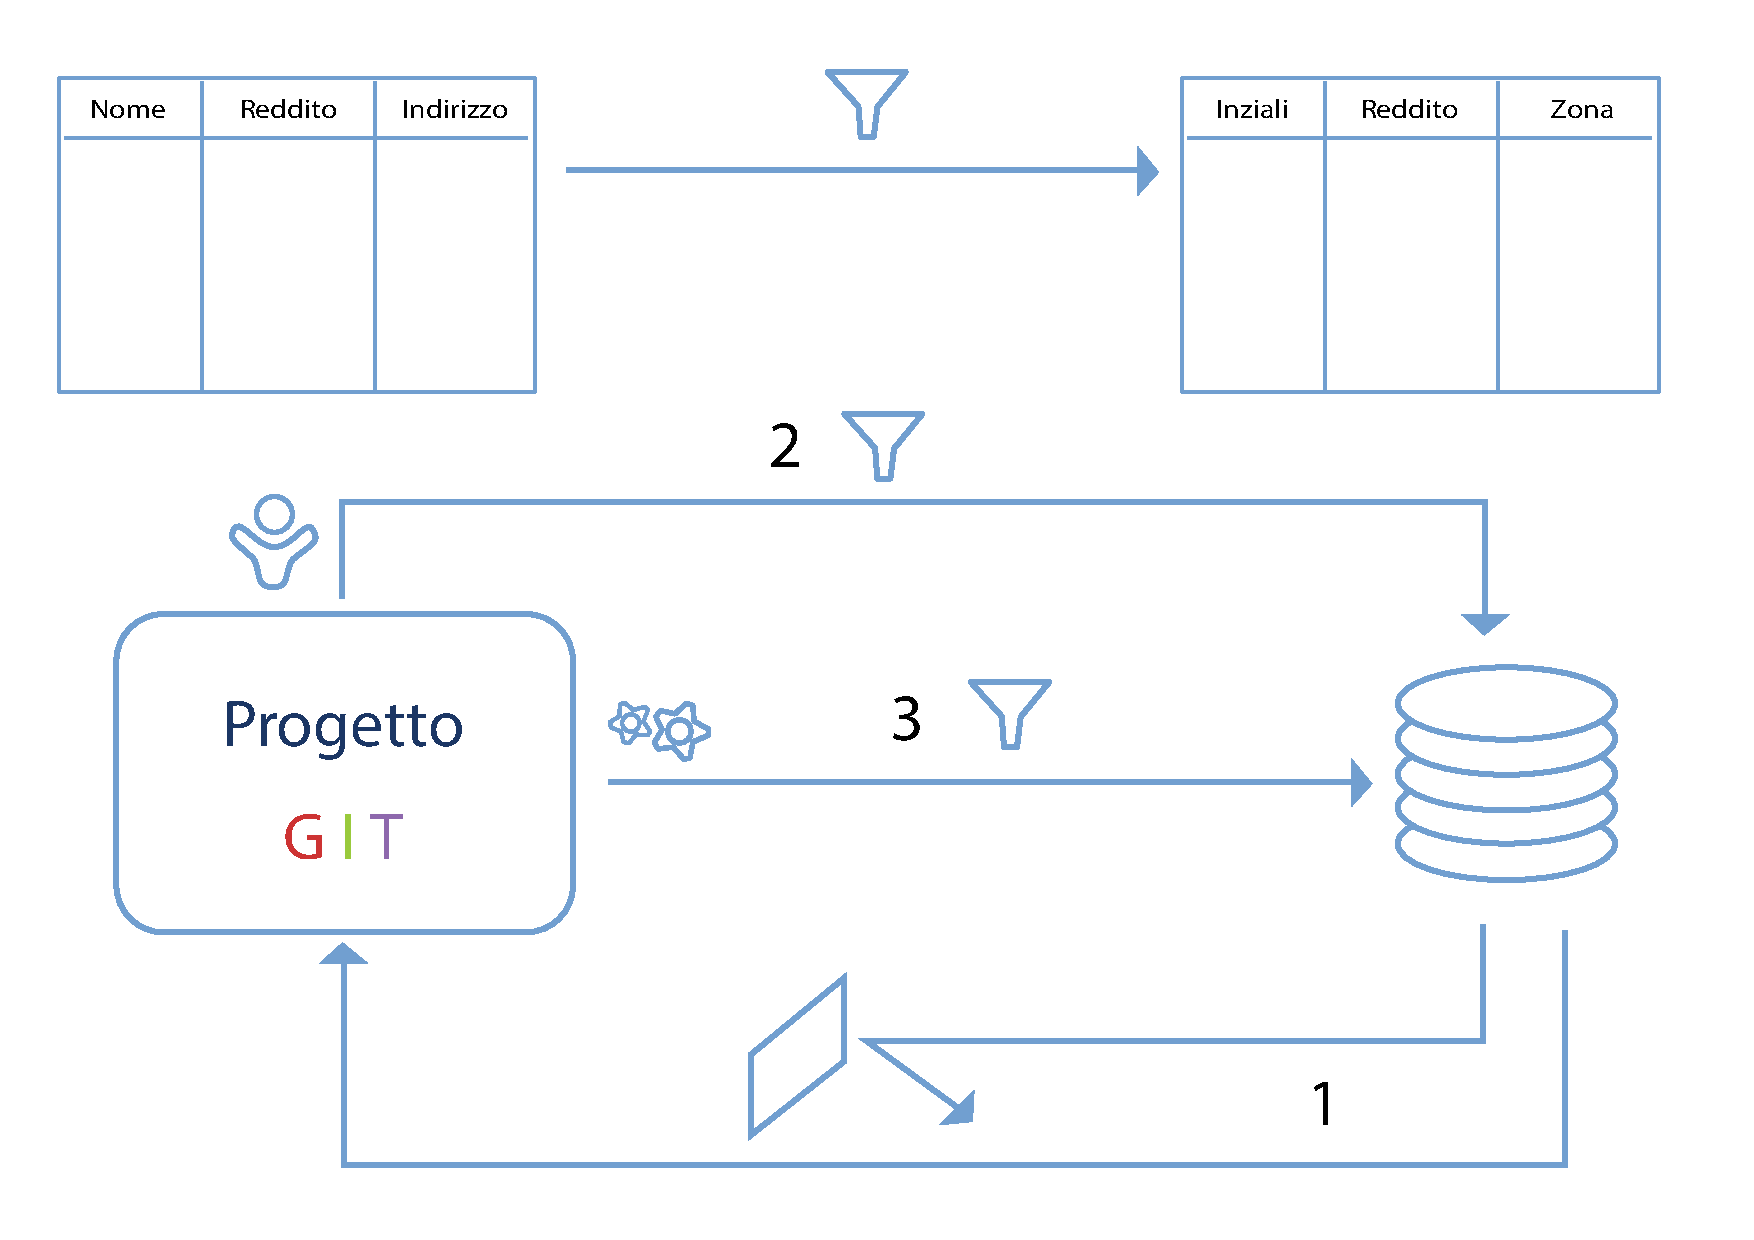
\includegraphics[scale=0.40]{img/git-ckan_clear} % requires the graphicx package
   \caption{Possibili soluzioni di integrazione tra GIT e il portale}
   \label{fig:git-ckan}
\end{figure}

\begin{enumerate}
\item Permettere alla piattaforma di accedere direttamente ai dati di GIT.
\item Effettuare periodicamente delle esportazioni dei dati da GIT per caricarle sulla piattaforma.
\item Effettuare l'aggiornamento dei dati sulla piattaforma ogni volta che vengono aggiornati su GIT in automatico.
\end{enumerate}

La prima soluzione presenta dei problemi di sicurezza, perch� per realizzarla bisogna modificare GIT creando un�interfaccia che permetta l'interrogazione ai dati dall'esterno. Ci� pu� diventare un problema nel momento in cui si creano delle API di interrogazioni generiche e quindi in alcune occasioni si finisce a violare la privacy degli utenti.

La seconda soluzione pu� essere applicata nei casi in cui le informazioni hanno una frequenza di aggiornamento rada, ma diventa impraticabile nel momento in cui i dati vengo aggiornati con una frequenza rilevante, in quando bisogna fare manualmente un aggiornamento ogni volta.

La soluzione vincente risulta quindi essere la terza. Questa comporta un controllo degli eventi sulla piattaforma GIT e l'esistenza di un sistema di aggiornamento automatizzato (senza intervento umano) sulla piattaforma Open Data.
Nell'ottica del riutilizzo del software, questa componente deve essere in grado di controllare eventuali aggiornamenti di GIT, di anonimizzare i dati e di inserirli nella piattaforma attraverso API.\\

%Catalogo e dizionario
Al fine di agevolare l'integrazione tra la piattaforma e applicazioni di terze parti si vuole rendere disponibile un \textbf{catalogo} contenente tutti i dataset e i relativi metadati. Con Metadati si intendono le informazioni riguardanti il singolo dataset quali il suo nome, la sua descrizione, il formato del file, la sua data di ultima modifica, il link a cui raggiungere la risorsa, ...

Si vuole inoltre rendere disponibile per ogni dataset il dizionario dei dati in esso contenuto. Ci� vuol dire che nel catalogo sar� presente anche l'informazione della tabella per ogni singolo dataset.

In questo modo � possibile interrogare il dataset sapendo a priori il tipo di dato che � contenuto in esso.\\

%Trigger e workflow
Si � scelto di utilizzare una piattaforma open source in accordo con il Comune di Vigevano e di conseguenza CKAN � stata la piattaforma sulla quale si � scelto di implementare i requisiti.
Al fine di rendere compatibile le modifiche apportate alla piattaforma CKAN tra le varie versioni della stessa si � deciso di analizzarlo come una �scatola nera�, senza mettere mano al codice sorgente di CKAN.

\begin{figure}[htbp]
   \centering
   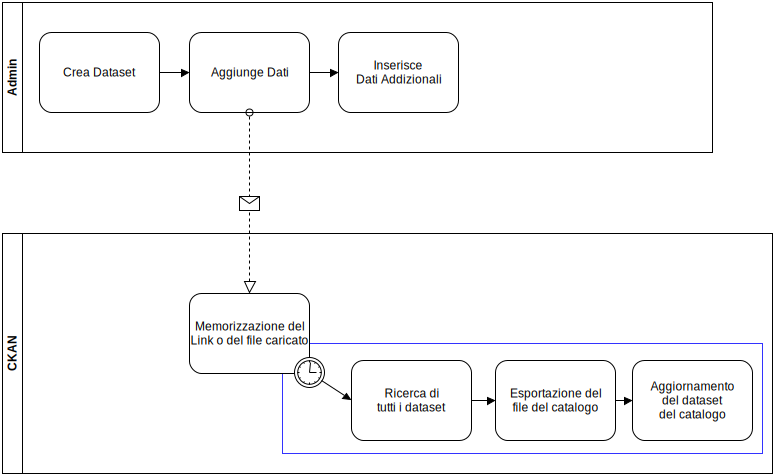
\includegraphics[scale=0.5]{img/workflow-creazione-dataset} % requires the graphicx package
   \caption{Workflow dell�aggiornamento del catalogo al momento dell�inserimento di un nuovo dataset}
   \label{fig:workflow}
\end{figure}

La progettazione del catalogo � quindi stata fatta come mostrato in fig. \ref{fig:workflow} inserendo un trigger (una procedura che viene eseguita in maniera automatica in coincidenza di un determinato evento) nella base di dati, il quale si attiva ad ogni aggiornamento nel database della tabella contenente i dataset, eseguendo una query che restituisce il catalogo (facendo un join tra diverse tabelle) e la esporta in formato CSV. Il file contenente il catalogo � esso stesso parte integrante della piattaforma essendo a sua volta un dataset.

	\section{Integrazione con Regione Lombardia}

\newpage %nuova pagina

%-------------------------------------------------------------------------

\chapter{Sviluppo-della-soluzione} 
	\section{Caricamento automatico}

	%\section{Dizionario dati}
\section{Catalogo dati}

%trigger, query, il flusso
Una volta che CKAN � stato popolato di dataset si � realizzato il catalogo dei dataset presenti.
Per fare ci� � stato necessario recuperare le informazioni contenute nel database e quindi le tabelle prese in esame sono state \texttt{package}, \texttt{resource} e \texttt{resource\_group}. La loro struttura � mostrata in figura \ref{fig:DB-design}:

\begin{figure}[htbp]
   \centering
   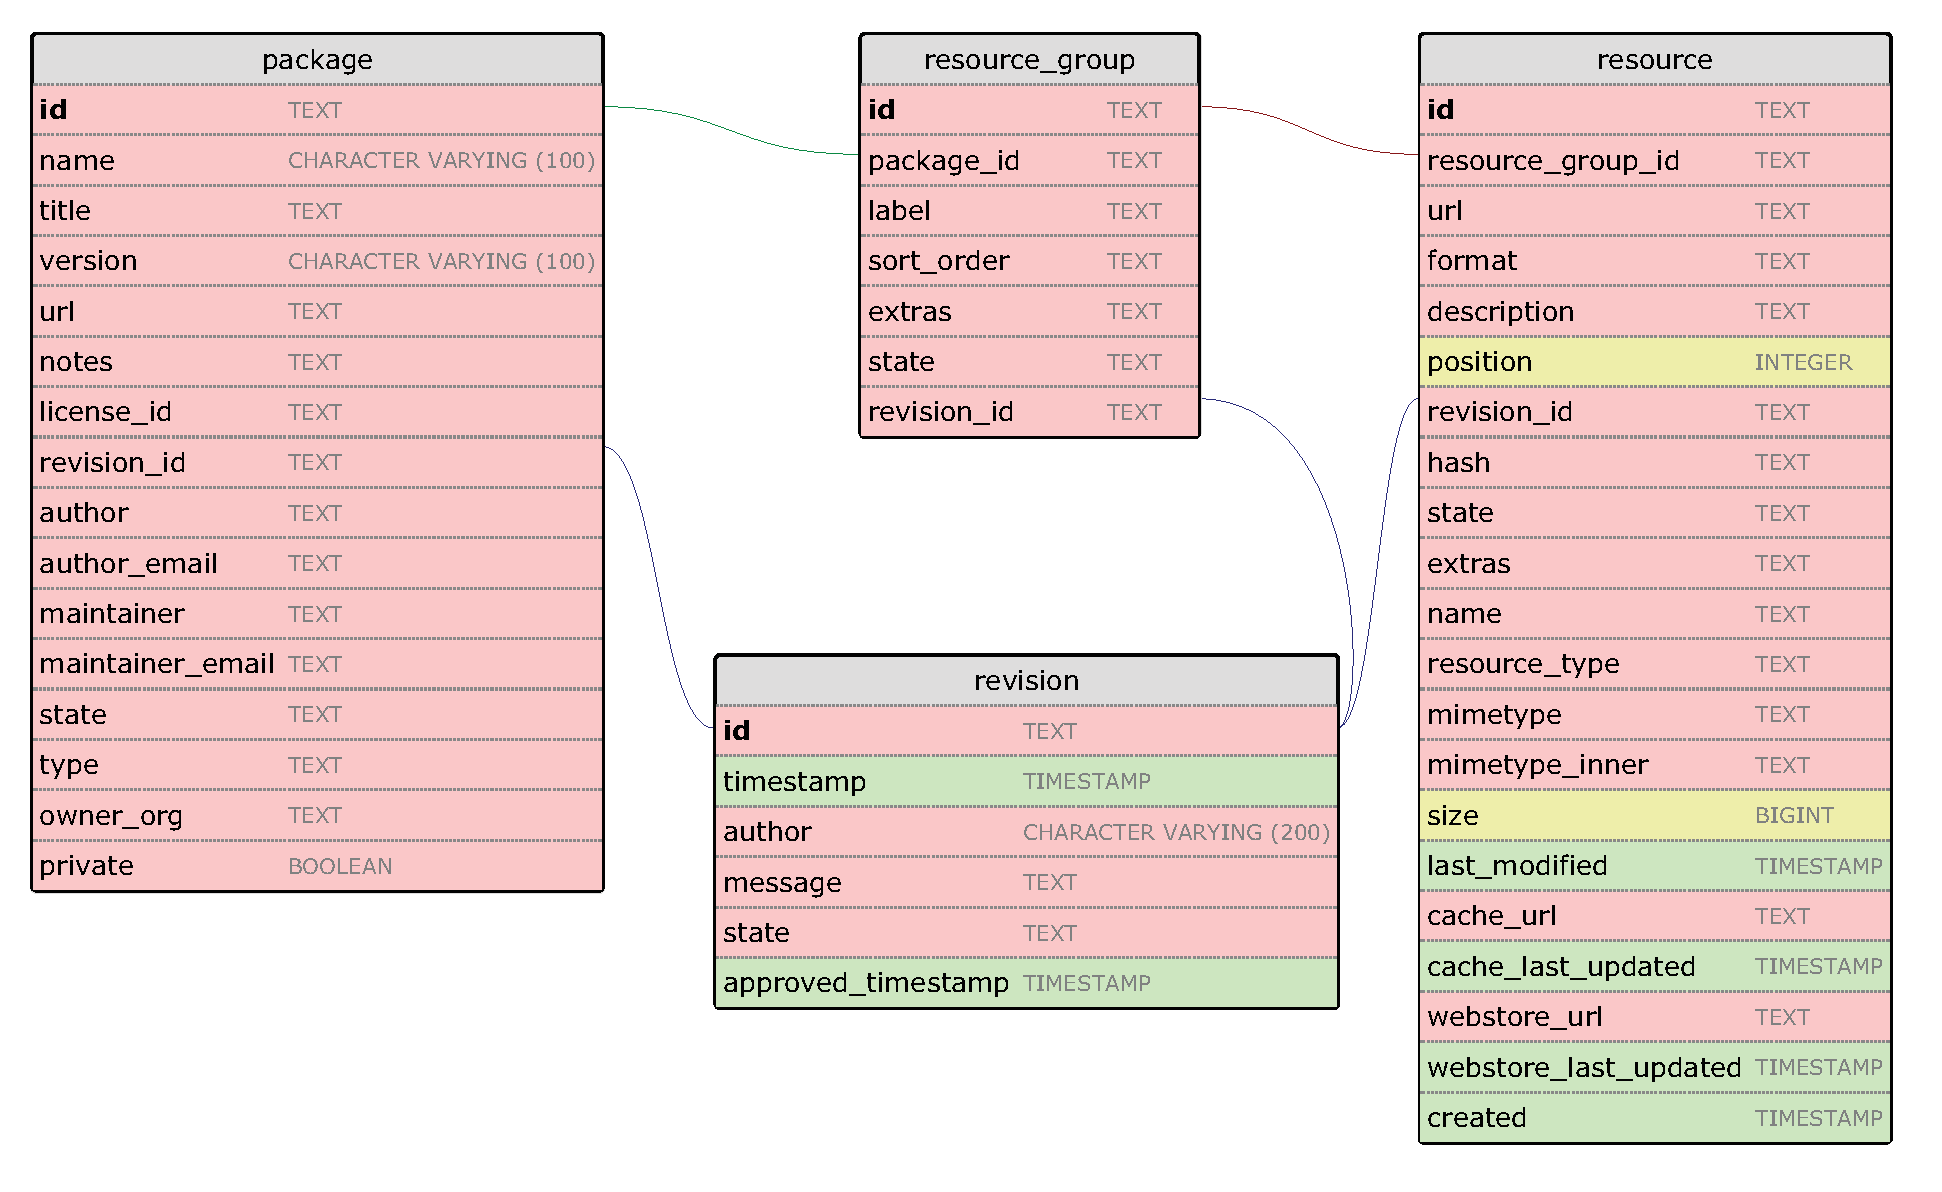
\includegraphics[scale=0.40]{img/DB-design2}
   \caption{Design DataBase}
   \label{fig:DB-design}
\end{figure}

Le informazioni sono presenti in tabelle differenti, ed � quindi stato necessario fare un JOIN tra le 3 tabelle e successivamente selezionare solo i campi di nostro interesse. Inoltre si sono tradotte le intestazioni delle colonne in italiano e si � creato un nuovo campo (link) concatenando l�url base della piattaforma con le informazioni presenti nel database.
%Per realizzare tutto ci� si � utilizzato la seguente query:\\
%{\indent{\footnotesize \verb$SELECT "name" AS "nome", "description" AS "descrizione", "url" AS "url",$}}\\
%{\indent{\footnotesize \verb$ "format" AS "formato", "last_modified" AS "ultima modifica",$}}\\
%{\indent{\footnotesize \verb$ "author" AS "autore", "author_email" AS "email autore",$}}\\
%{\indent{\footnotesize \verb$ "maintainer" AS "manutentore", "maintainer_email" AS "email manutentore",$}}\\
%{\indent{\footnotesize \verb$ CONCAT('http://localhost/dataset/',url_name,'/resource/',url_id) AS "link"$}}\\
%{\indent{\footnotesize \verb$FROM	($}}\\
%{\indent{\footnotesize \verb$ SELECT	"name", "description", "url", "format", "last_modified",$}}\\
%{\indent{\footnotesize \verb$   "resource_group_id", "package_id", resource.id AS "url_id"$}}\\
%{\indent{\footnotesize \verb$ FROM	"resource_group"$}}\\
%{\indent{\footnotesize \verb$ JOIN	"resource"$}}\\
%{\indent{\footnotesize \verb$ ON	resource_group.id=resource.resource_group_id$}}\\
%{\indent{\footnotesize \verb$ WHERE	"name"<>'datacatalog.csv'$}}\\
%{\indent{\footnotesize \verb$ ) AS "resource"$}}\\
%{\indent{\footnotesize \verb$JOIN	($}}\\
%{\indent{\footnotesize \verb$ SELECT	"id", "author", "author_email", "maintainer", "maintainer_email",$}}\\
%{\indent{\footnotesize \verb$  "name" AS "url_name"$}}\\
%{\indent{\footnotesize \verb$ FROM	"package") AS "package"$}}\\
%{\indent{\footnotesize \verb$ON	resource.package_id=package.id$}}\\
%{\indent{\footnotesize \verb$ORDER BY "last_modified" DESC;$}}\\

Ci� � stato realizzato attraverso una query, il cui risultato � stato esportato in un file in formato CSV (comma-separated values). Si � voluto salvare il file in una posizione che fosse poi recuperabile dal web server, di conseguenza si � scelto di salvarlo nella sua root. Ci� � possibile utilizzando il comando \textit{Copy} dopo aver acceduto al database PostgreSQL:\\

\shellcmd{sudo psql -h localhost -U ckanuser ckan\_default}
{\indent\indent{\footnotesize \verb$\Copy ($}}\\
\\
\centerline{\texttt{...QUERY...}}\\
\\
{\indent\indent{\footnotesize \verb$) To '/usr/lib/ckan/default/src/ckan/ckan/public/datacatalog.csv'$}}\\
{\indent\indent{\footnotesize \verb$With CSV HEADER$}}\\

  
Successivamente, per automatizzare il processo di creazione del catalogo ad ogni nuovo inserimento di un dataset in CKAN, sono stati creati una funzione ed un trigger.
La funzione non fa altro che eseguire l'esportazione della query in CSV nella posizione prestabilita:\\

{\indent{\footnotesize \verb#CREATE FUNCTION create_datacatalog ()#}}\\
{\indent{\footnotesize \verb#RETURNS trigger#}}\\
{\indent{\footnotesize \verb#AS $create_datacatalog$#}}\\
{\indent{\footnotesize \verb#BEGIN EXECUTE '#}}\\
{\indent{\footnotesize \verb#Copy (SELECT "name" AS "nome", "description" AS "descrizione", "url" AS#}}\\
{\indent{\footnotesize \verb# "url", "format" AS "formato", "last_modified" AS "ultima modifica",#}}\\
{\indent{\footnotesize \verb# "author" AS "autore", "author_email" AS "email autore", "maintainer"#}}\\
{\indent{\footnotesize \verb# AS "manutentore", "maintainer_email" AS "email manutentore" FROM (#}}\\
{\indent{\footnotesize \verb# SELECT "name", "description", "url", "format", "last_modified",#}}\\
{\indent{\footnotesize \verb# "resource_group_id", "package_id", resource.id AS "url_id"#}}\\
{\indent{\footnotesize \verb# FROM "resource_group" JOIN "resource"#}}\\
{\indent{\footnotesize \verb# ON resource_group.id=resource.resource_group_id) AS "resource"#}}\\
{\indent{\footnotesize \verb# JOIN (SELECT "id", "author", "author_email", "maintainer",#}}\\
{\indent{\footnotesize \verb# "maintainer_email", "name" AS "url_name" FROM "package") AS "package"#}}\\
{\indent{\footnotesize \verb# ON resource.package_id=package.id ORDER BY "last_modified" DESC)#}}\\
{\indent{\footnotesize \verb# To ''/usr/lib/ckan/default/src/ckan/ckan/public/datacatalog.csv''#}}\\
{\indent{\footnotesize \verb# With CSV HEADER;#}}\\
{\indent{\footnotesize \verb#';#}}\\
{\indent{\footnotesize \verb#RETURN NEW;#}}\\
{\indent{\footnotesize \verb#END;#}}\\
{\indent{\footnotesize \verb#$create_datacatalog$#}}\\
{\indent{\footnotesize \verb#LANGUAGE plpgsql;#}}\\
\\
Mentre invece il trigger si attiva ad ogni modifica della tabella \texttt{resource} e invoca la funzione:\\

{\indent{\footnotesize \verb#CREATE TRIGGER datacatalog_update#}}\\
{\indent{\footnotesize \verb#AFTER insert OR update#}}\\
{\indent{\footnotesize \verb#ON resource#}}\\
{\indent{\footnotesize \verb#FOR EACH ROW#}}\\
{\indent{\footnotesize \verb#EXECUTE PROCEDURE create_datacatalog();#}}\\
\\

Infine per rendere possibile la modifica del file \texttt{datacatalog.csv} da parte del web server si � assegnato al file i permessi di scrittura all'utente \texttt{ckan}:\\

\shellcmd{chown ckan /usr/lib/ckan/default/src/ckan/ckan/public/datacatalog.csv}
\shellcmd{chmod 755 /usr/lib/ckan/default/src/ckan/ckan/public/datacatalog.csv}

% vedere: http://pleasemakeanote.blogspot.it/2009/08/how-to-highlight-text-in-latex.html

%   modificare permessi ckanuser, ma se creassi i 2 cos� come superuser direttamente?
% ckan@ckan-virtual-machine:~$ sudo -u postgres psql
% psql (9.1.9)
% Type "help" for help.

% postgres=# alter role ckanuser SUPERUSER;
% ALTER ROLE
% postgres=# 
\todo{Nella procedura di configurazione ho anche fatto �alter role ckanuser SUPERUSER� in postresql altrimenti quando veniva lanciato il frigger la funzione non riusciva ad esportare le informazioni. Prima di inserirlo volevo riprovare facendo per� login al DB non con cknauser, ma come l�utente superuser (non mi ricordo se esiste) e creare con quello il trigger e la funzione.}

\section{Dizionario dati}
Nelle intenzioni dello sviluppo della piattaforma si � cercato di aggiungere nel catalogo anche le informazioni sul tipo di dato contenuto in ogni singolo dataset. In pratica si voleva inserire un ulteriore colonna nel catalogo contenente le intestazioni della tabella del dataset.
Purtroppo non si � trovata una soluzione per realizzare questa feature in quanto non si � trovato il modo di recuperare le informazioni presenti nei due differenti database che sono relazionati come mostrato in figura \ref{fig:DBs-ckan}:

\begin{figure}[htbp]
   \centering
   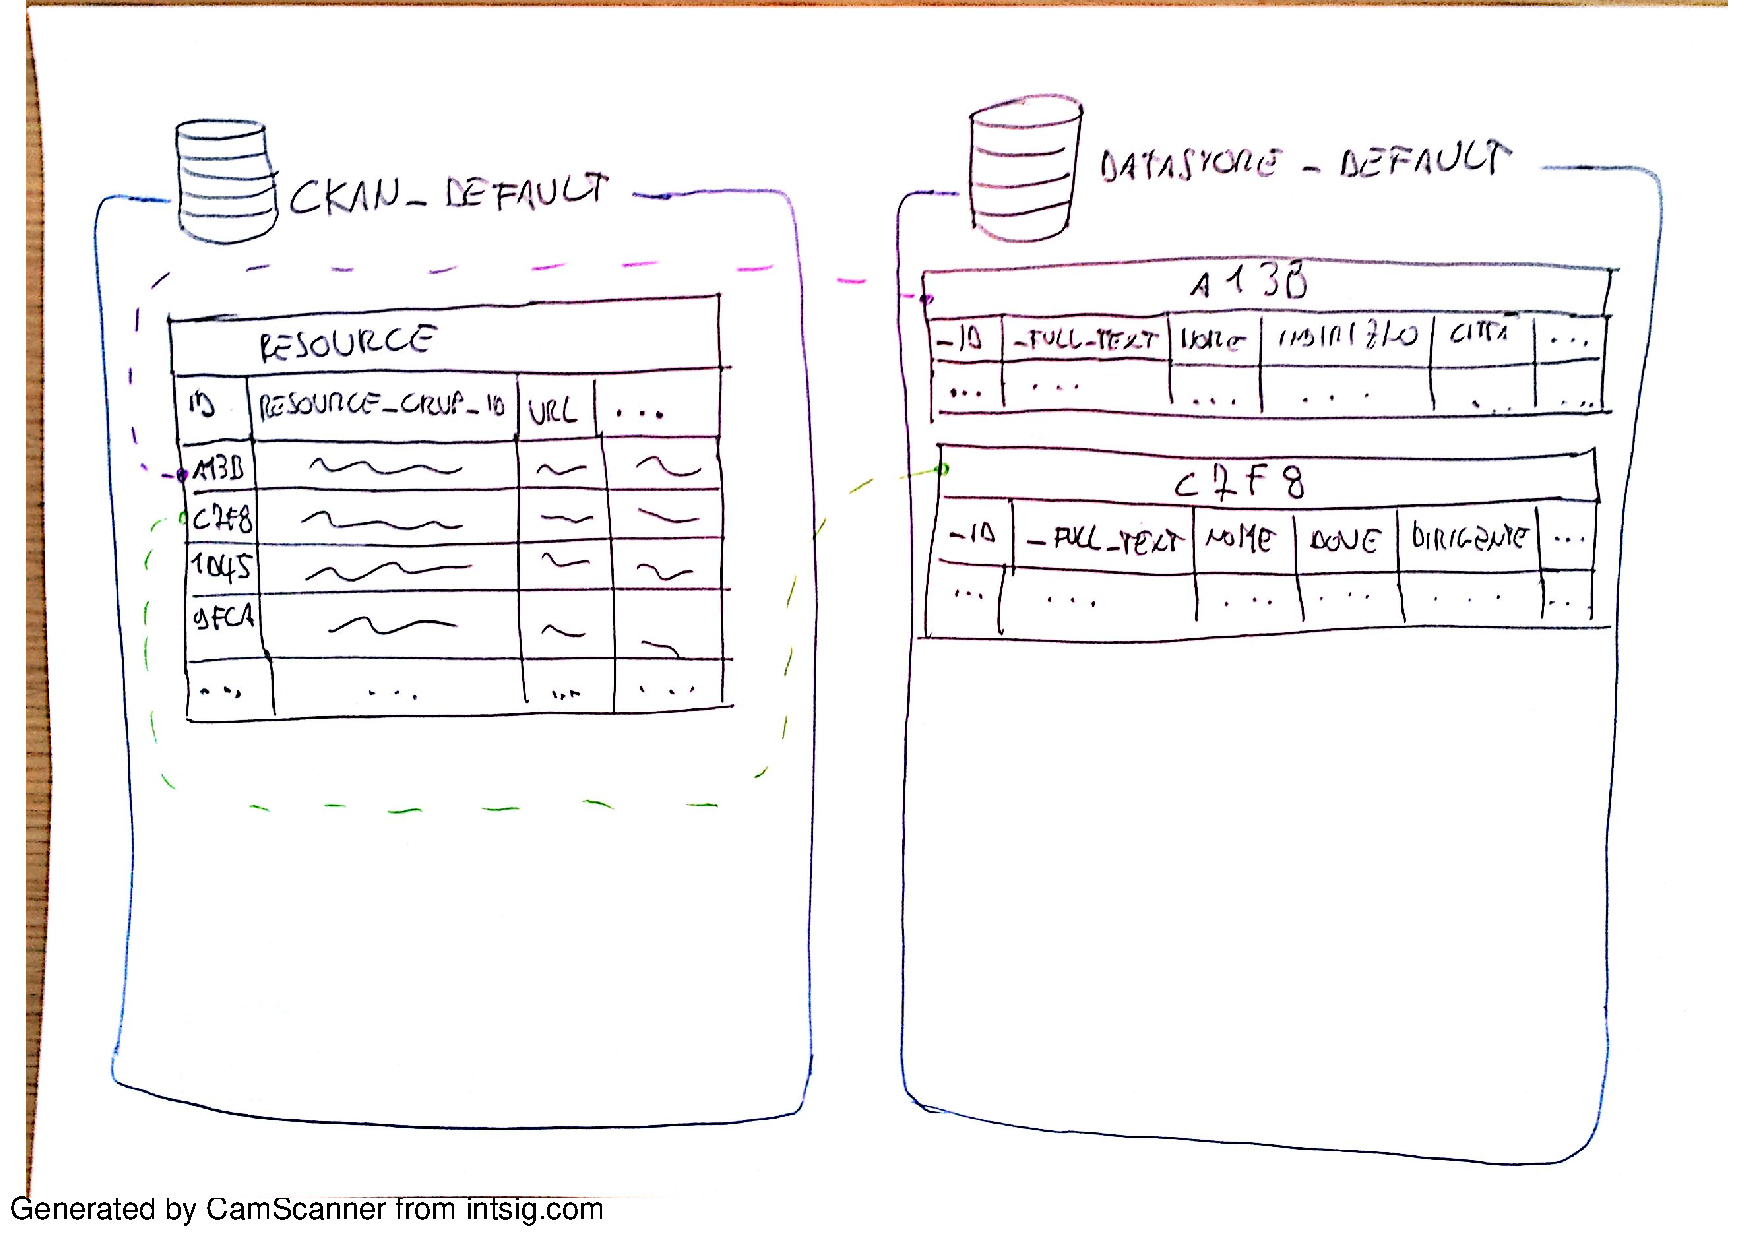
\includegraphics[scale=0.35]{img/DBs-ckan}
   \caption{relazione tra le tabelle dei DataBase utilizzati da CKAN}
   \label{fig:DBs-ckan}
\end{figure}

L�impossibilit� di recuperare l�intestazione delle tabelle del database \texttt{datastore\_default} una volta conosciuto il valore nel campo \texttt{id} dei singoli elementi presenti nella tabella \texttt{resource} del database \texttt{ckan\_default} non ha quindi al momento permesso la creazione del dizionario dati.
	\section{Blueprint}

Per realizzare l�integrazione tra la piattaforma CKAN realizzata per il Comune di Vigevano e la piattaforma Socrata utilizzata da Regione Lombardia si � pensato di importare il catalogo della prima nella seconda.\\

Dalla documentazione presente su Socrata si � ipotizzato di utilizzare quanto descritto alla pagina \url{http://dev.socrata.com/publishers/importing}.

L�importazione dei dati viene eseguita come un processo in due fasi. In primo luogo, il file di dati in s� viene caricato tramite l'API, e viene poi analizzato per determinare il tipo di dati che esso contiene. I risultati di tale analisi vengono restituiti, dopodich� � possibile apportare modifiche al modo in cui l'importatore interpreta i dati. A questo punto si invia il progetto di importazione risultante, e a questo punto inizia il processo di importazione vero e proprio.

Al momento questa soluzione non � stata ancora sperimentata, mancando i tempi tecnici di realizzazione.
\newpage %nuova pagina

%-------------------------------------------------------------------------

\chapter{Utilizzo della piattaforma}

Dopo la prima installazione la piattaforma si presenta, come mostrato in figura \ref{fig:demo-1-ckan-vergine}, con un�interfaccia sobria e  pronta a contenere i dataset che varranno caricati.

\begin{figure}[htbp]
   \centering
   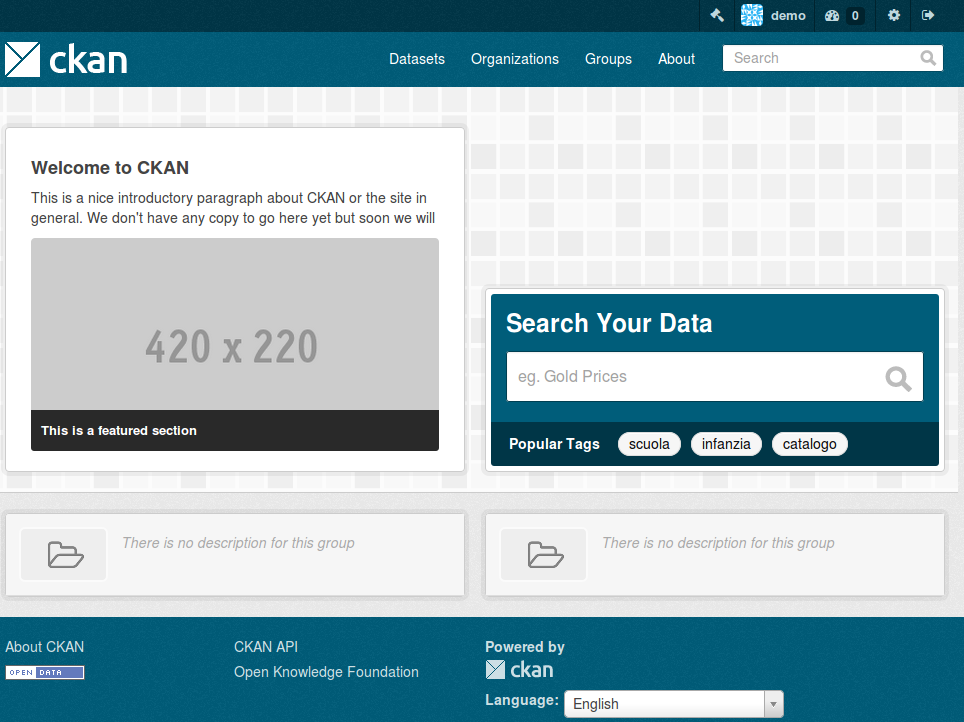
\includegraphics[scale=0.42]{img/demo-1-ckan-vergine}
   \caption{Aspetto di CKAN appena installato}
   \label{fig:demo-1-ckan-vergine}
\end{figure}

\newpage
Navigando alla voce di men� �Dataset� � possibile vedere l�elenco dei dataset disponibili, ma anche crearne uno nuovo attraverso il pulsante presente in alto a destra (figura \ref{fig:demo-2-ckan-creazione-dataset}).

\begin{figure}[htbp]
   \centering
   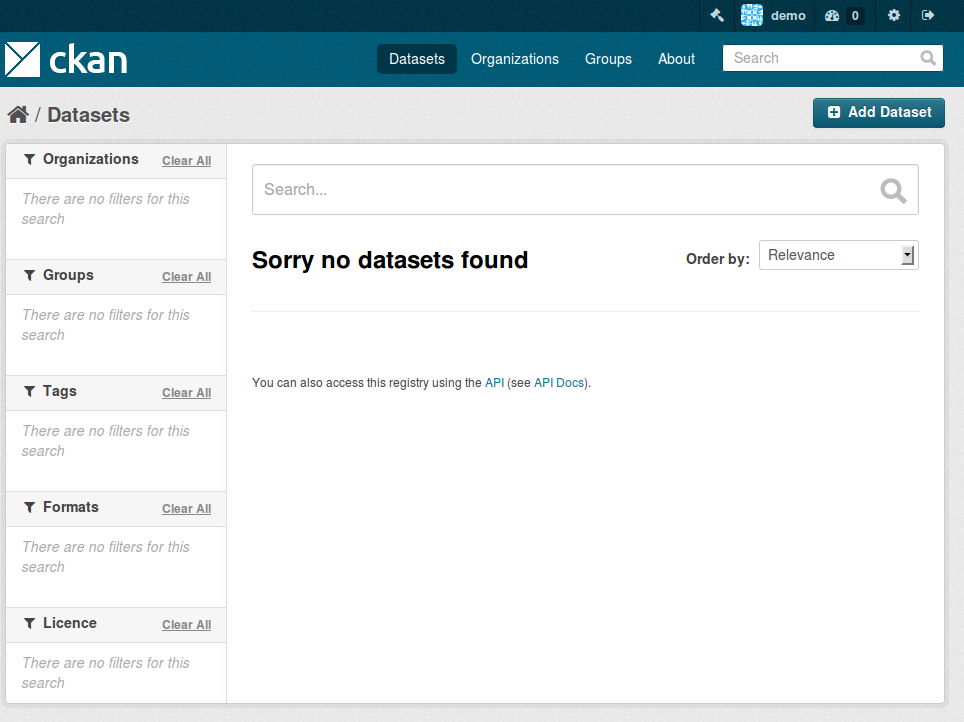
\includegraphics[scale=0.42]{img/demo-2-ckan-creazione-dataset}
   \caption{Elenco dei Dataset vuoto}
   \label{fig:demo-2-ckan-creazione-dataset}
\end{figure}

\newpage
L�inserimento di un nuovo Dataset inizia con la richiesta di inserimento delle meta-informazioni necessarie alla sua identificazione (figura \ref{fig:demo-3-ckan-primo-passo}), ovvero il titolo e la descrizione; l�utente pu� anche decidere di inserire opzionalmente alcuni tag per facilitarne la ricerca e la licenza da un elenco predefinito.

\begin{figure}[htbp]
   \centering
   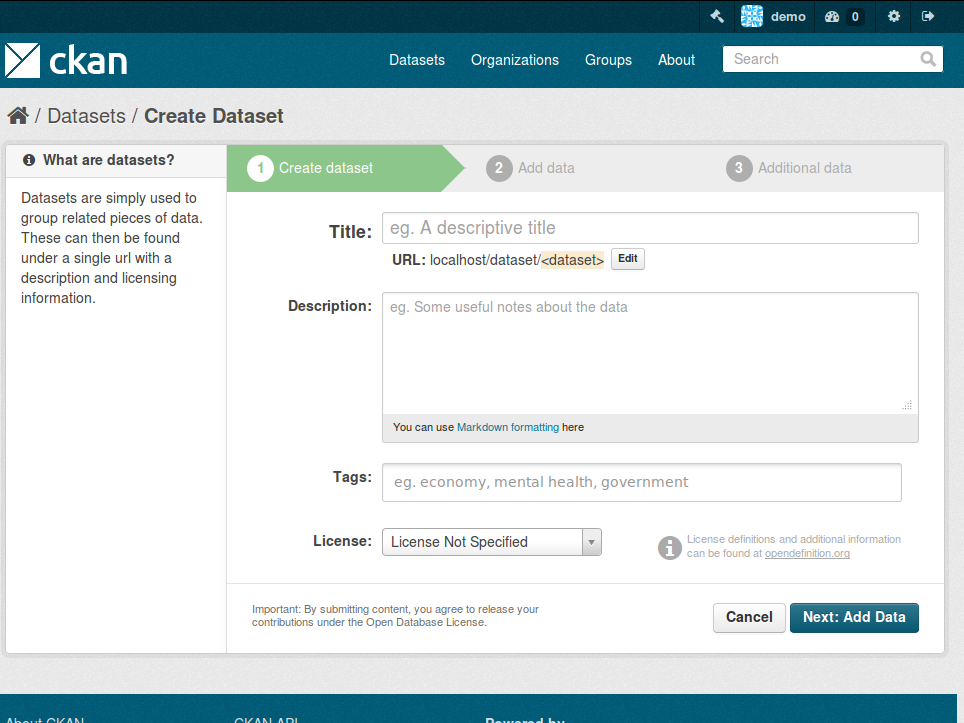
\includegraphics[scale=0.42]{img/demo-3-ckan-primo-passo}
   \caption{Definizione dei metadati durante la creazione di un dataset}
   \label{fig:demo-3-ckan-primo-passo}
\end{figure}

\newpage
Ad esempio possiamo inseriti i metadati necessari alla creazione del catalogo (figura \ref{fig:demo-3-ckan-primo-passo-condati}) per poi passare all�aggiunta dei dati veri e prorpi.

\begin{figure}[htbp]
   \centering
   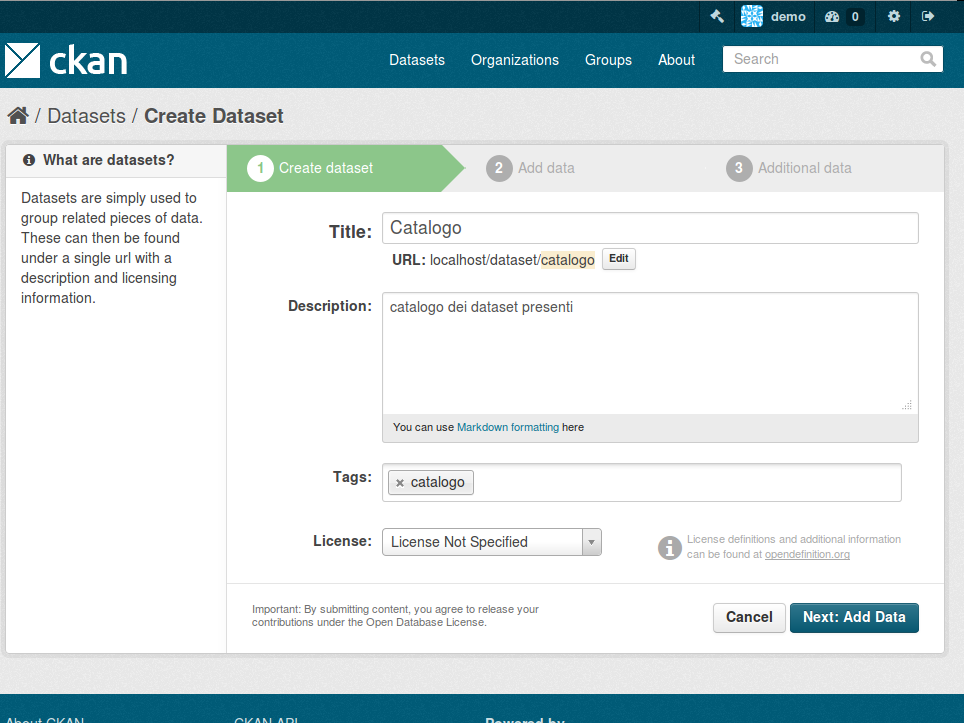
\includegraphics[scale=0.42]{img/demo-3-ckan-primo-passo-condati}
   \caption{Inserimento metadati del catalogo}
   \label{fig:demo-3-ckan-primo-passo-condati}
\end{figure}

\newpage
Nel secondo passaggio � possibile linkare un file o una risorsa esterna e specificare il nome e la descrizione che verranno utilizzati nella piattaforma (figura \ref{fig:demo-4-ckan-secondo-passo-condati}). Il formato del file viene identificato automaticamente, in caso ci� non avvenga � possibile inserirlo manualmente.

\begin{figure}[htbp]
   \centering
   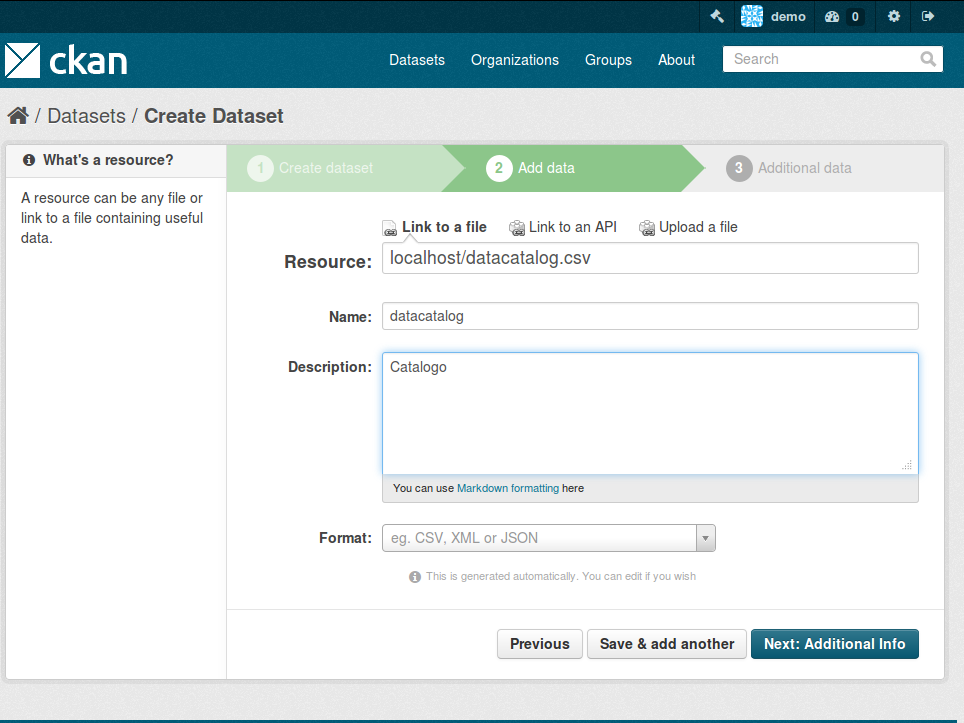
\includegraphics[scale=0.42]{img/demo-4-ckan-secondo-passo-condati}
   \caption{Inserimento risorsa nel dataset}
   \label{fig:demo-4-ckan-secondo-passo-condati}
\end{figure}

\newpage
In alternativa, una volta attivato il File Store � possibile caricare un file dal proprio computer in modo che venga memorizzato nel server (figura \ref{fig:demo-7-upload-scuola}). Un messaggio ci avvertir� del successo dell�upload o dell�eventuale fallimento nella parte alta dello schermo.

\begin{figure}[htbp]
   \centering
   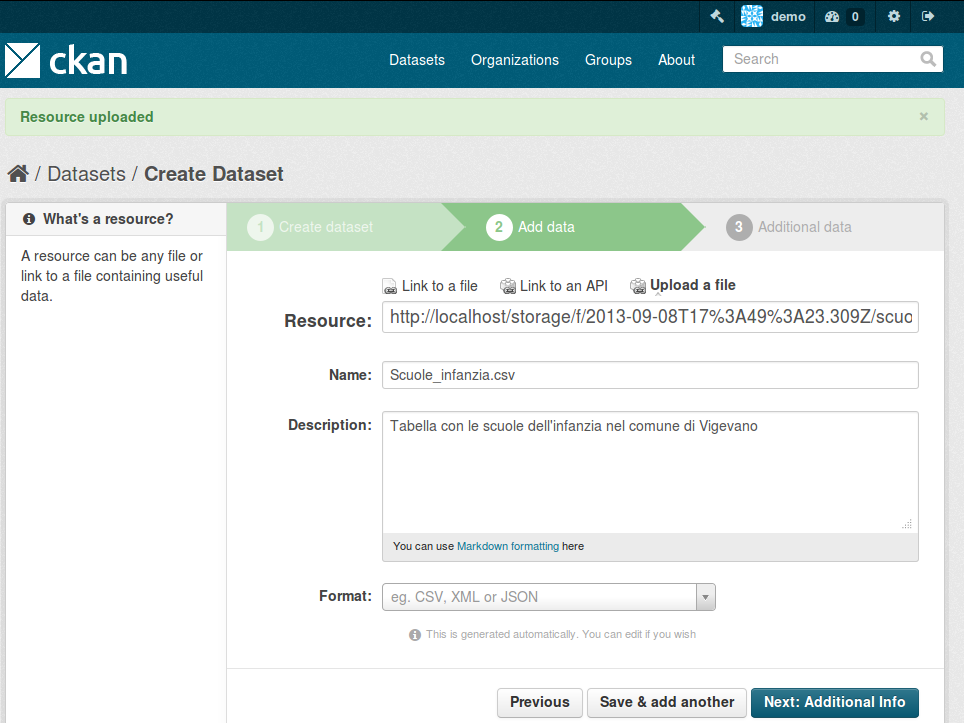
\includegraphics[scale=0.42]{img/demo-7-upload-scuola}
   \caption{Upload fine in CKAN}
   \label{fig:demo-7-upload-scuola}
\end{figure}

\newpage
Infine � possibile aggiungere ulteriori informazioni riguardanti l�autore dei dati e il manutentore (colui che si preoccupa di aggiornare il dataset nel tempo). Inoltre � possibile assegnare in dataset ad un gruppo (figura \ref{fig:demo-5-ckan-terzo-passo-condati}).

\begin{figure}[htbp]
   \centering
   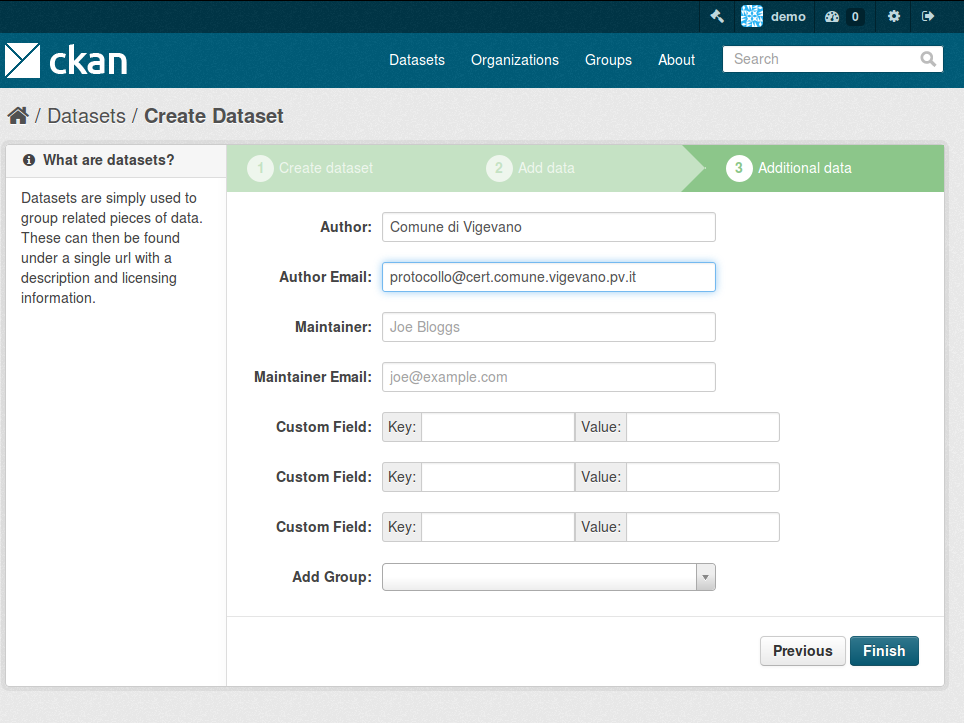
\includegraphics[scale=0.42]{img/demo-5-ckan-terzo-passo-condati}
   \caption{Inserimento dati addizionali del dataset}
   \label{fig:demo-5-ckan-terzo-passo-condati}
\end{figure}

\newpage
A questo punto ci viene mostrato il dataset con tutte le informazioni che abbiamo inserito (figura \ref{fig:demo-6-ckan-catalogo-vuoto}). Finch� il DataStorer non entra in funzione la preview non sar� disponibile.

\begin{figure}[htbp]
   \centering
   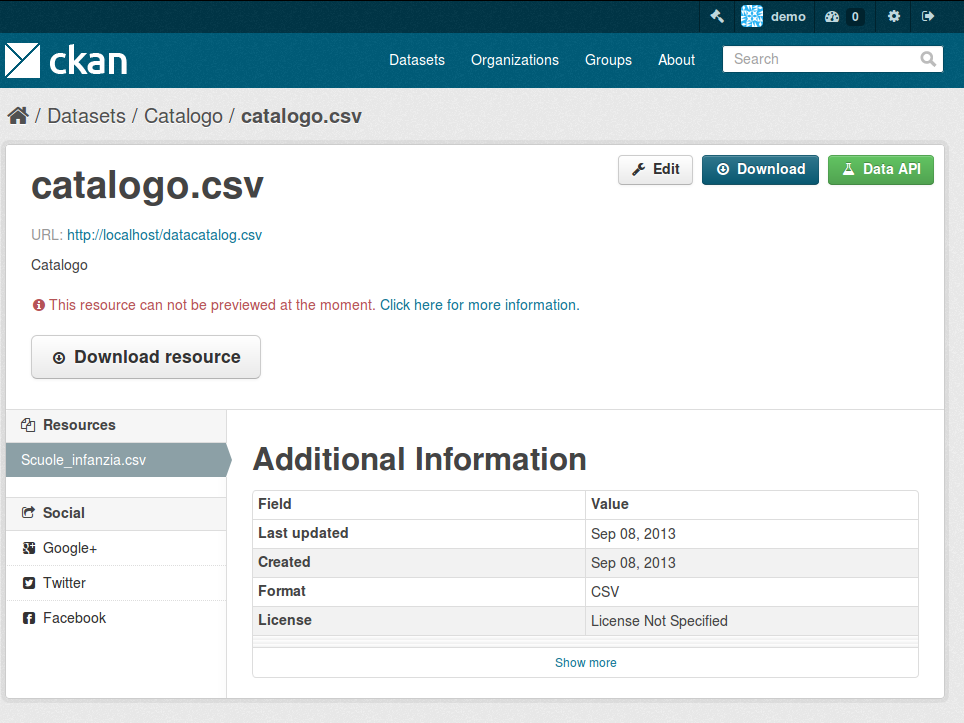
\includegraphics[scale=0.42]{img/demo-6-ckan-catalogo-vuoto}
   \caption{Dataset appena caricato, il DataStorer non � ancora entrato in funzione}
   \label{fig:demo-6-ckan-catalogo-vuoto}
\end{figure}

\newpage
Una volta che il file sar� processato e i dati contenuti nel dataset saranno salvati nel DataStore e la pagina si presenter� come mostrato in figura \ref{fig:demo-9-dataset-preview}.

\begin{figure}[htbp]
   \centering
   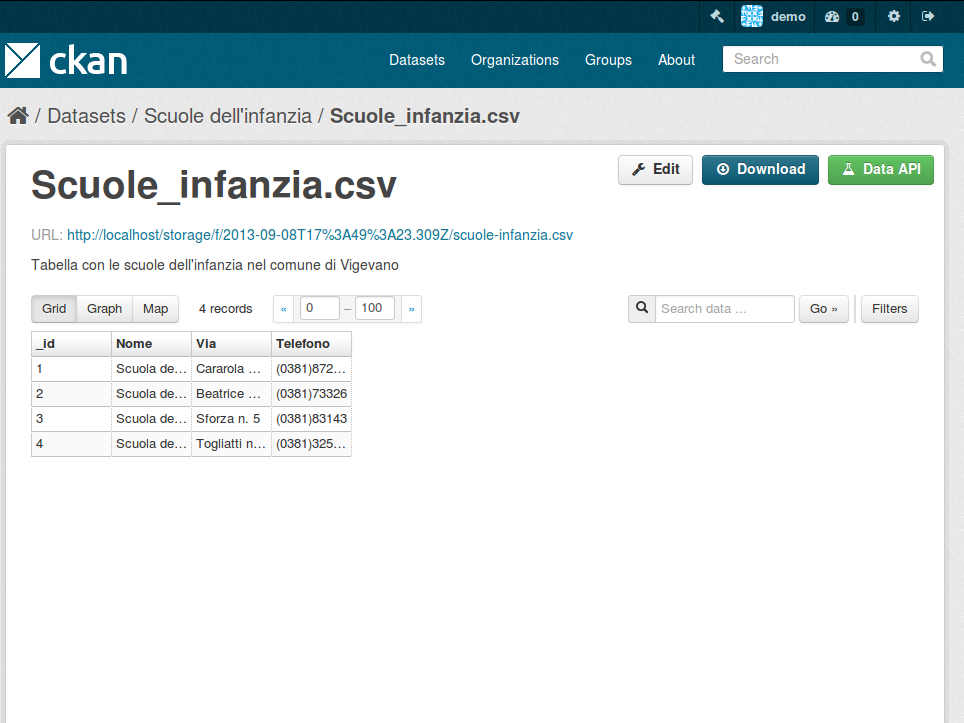
\includegraphics[scale=0.42]{img/demo-9-dataset-preview}
   \caption{Dataset con le informazioni memorizzato nel DataStore}
   \label{fig:demo-9-dataset-preview}
\end{figure}

\newpage
L�interfaccia grafica � personalizzabile rispetto alle esigenze e nel nostro caso � stata adattata per il Comune di vigevano (figura \ref{fig:demo-10-home-vigevano}).

\begin{figure}[htbp]
   \centering
   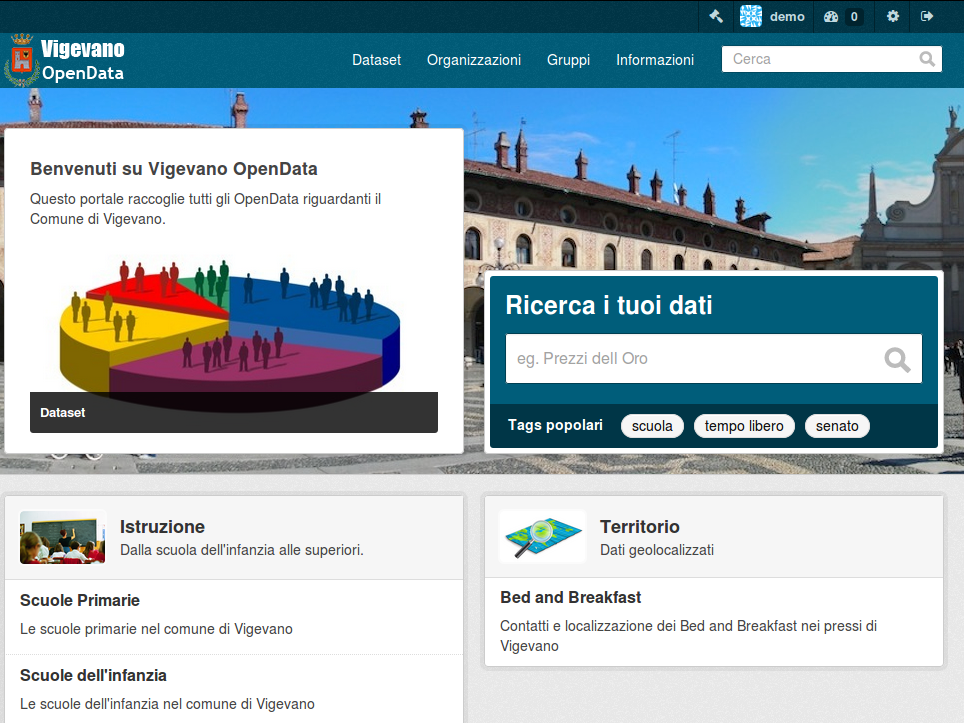
\includegraphics[scale=0.42]{img/demo-10-home-vigevano}
   \caption{Homepage di CKAN realizzato per il Comune di Vigevano}
   \label{fig:demo-10-home-vigevano}
\end{figure}

\newpage
Come mostrato in figura \ref{fig:demo-11-gruppi} � possibile suddividere i dataset per gruppi tematici, una funzione molto apprezzata dagli utenti che ricercano le informazioni di una determinata categoria.

\begin{figure}[htbp]
   \centering
   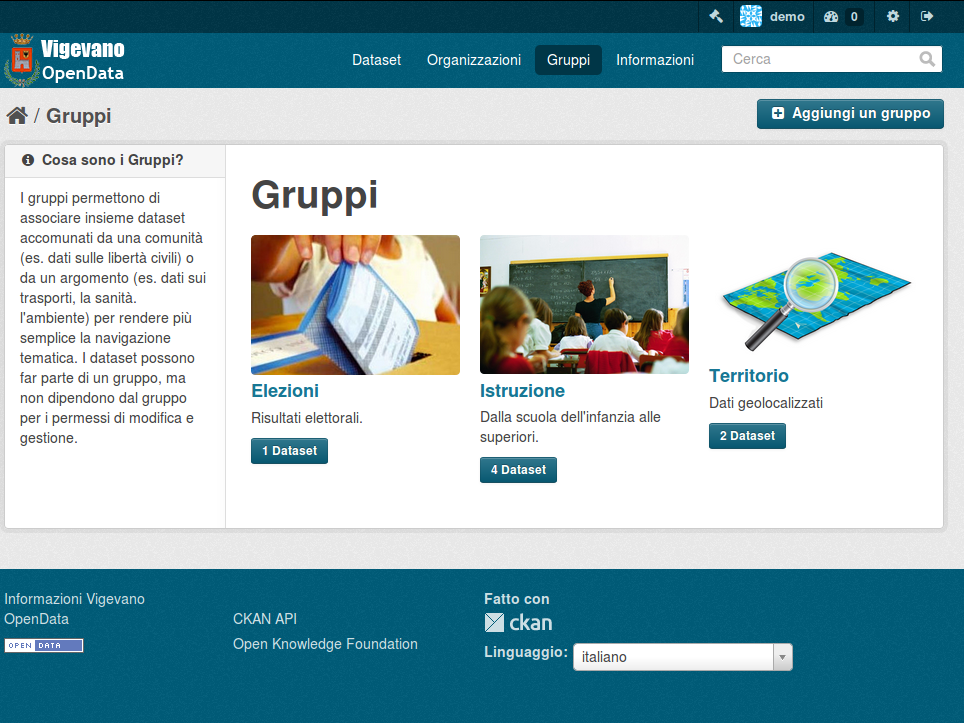
\includegraphics[scale=0.42]{img/demo-11-gruppi}
   \caption{Elenco dei gruppi di dataset disponibili}
   \label{fig:demo-11-gruppi}
\end{figure}

\newpage
Una volta entrati nella pagina di un gruppo viene presentato l�elenco dei dataset disponibili con al relativa descrizione e formato (figura \ref{fig:demo-12-gruppo-dettaglio}).

\begin{figure}[htbp]
   \centering
   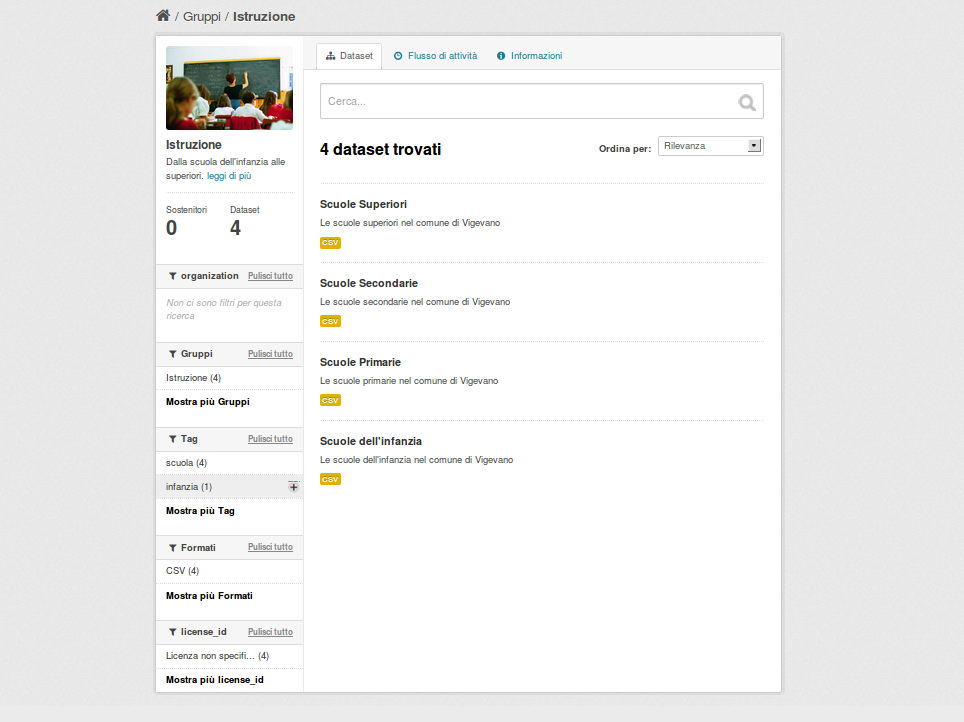
\includegraphics[scale=0.42]{img/demo-12-gruppo-dettaglio}
   \caption{Dettaglio dei dataset di un singolo gruppo}
   \label{fig:demo-12-gruppo-dettaglio}
\end{figure}


\newpage
I dati contenuti in un datset possono essere visualizzati in forma tabellare, dove � possibile ricercare una determinata informazione attraverso il campo di ricerca a destra sopra la tabella oppure attraverso i filtri (figura \ref{fig:demo-13-dataset-tabella}).

\begin{figure}[htbp]
   \centering
   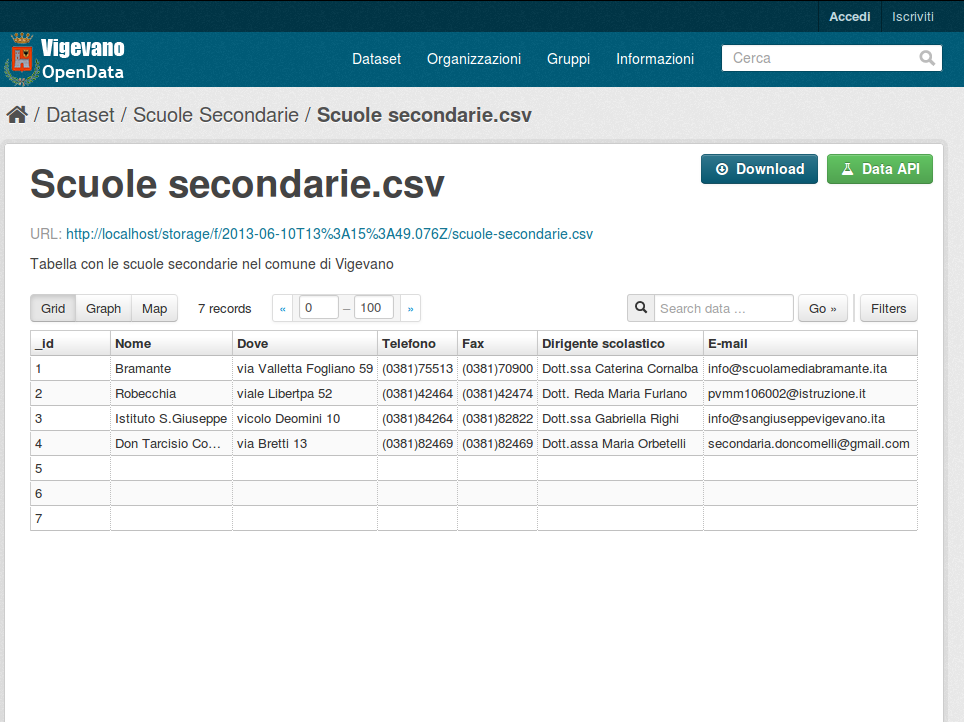
\includegraphics[scale=0.42]{img/demo-13-dataset-tabella}
   \caption{Visuale tabellare di un dataset}
   \label{fig:demo-13-dataset-tabella}
\end{figure}

\newpage
In caso esista una dipendenza tra due colonne � possibile visualizzare le informazioni attraverso dei grafici di vario tipo, ad esempio come grafico a punti o come grafico a barre (figura \ref{fig:demo-13-dataset-barre}).

\begin{figure}[htbp]
   \centering
   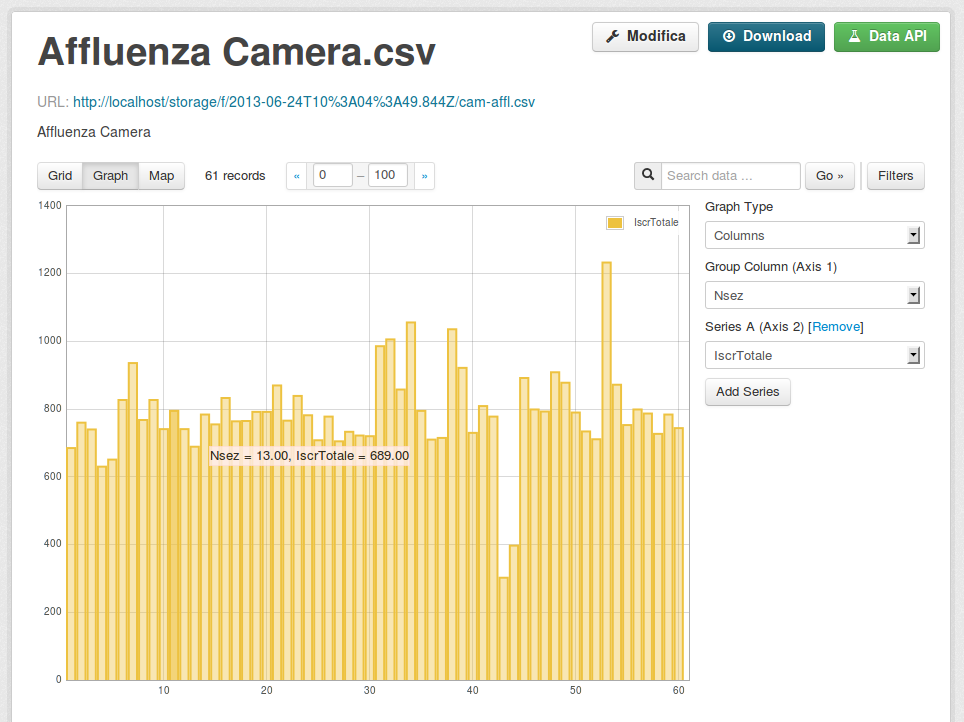
\includegraphics[scale=0.42]{img/demo-13-dataset-barre}
   \caption{Visuale a grafico di un dataset}
   \label{fig:demo-13-dataset-barre}
\end{figure}


\newpage
Infine in caso di dati geolocalizzati � possibile �mapparli� su una cartina (figura \ref{fig:demo-13-dataset-cartina}) di MapQuest. Ci� risulta veramente intuitivo per gli utenti finali.

\begin{figure}[htbp]
   \centering
   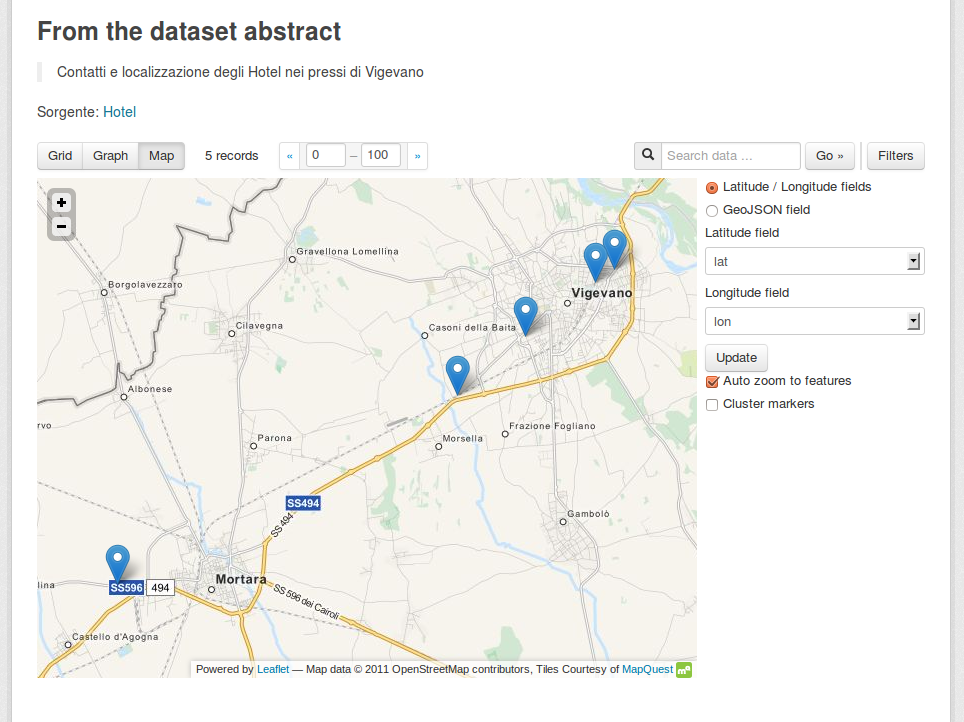
\includegraphics[scale=0.42]{img/demo-13-dataset-cartina}
   \caption{Visuale geolocalizzata di un dataset}
   \label{fig:demo-13-dataset-cartina}
\end{figure}

\newpage
Inoltre clickando su uno dei marcatori della cartina si visualizzano tutte le informazioni disponibili nel dataset relative al punto selezionato (figura \ref{fig:demo-13-dataset-cartina-dettaglio}).

\begin{figure}[htbp]
   \centering
   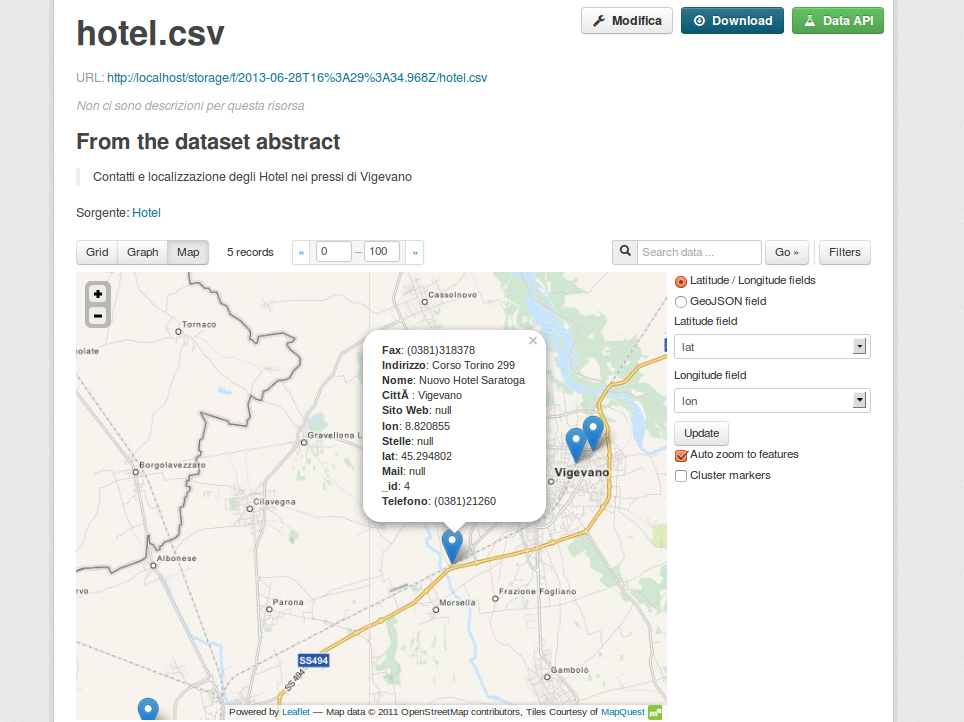
\includegraphics[scale=0.42]{img/demo-13-dataset-cartina-dettaglio}
   \caption{Dettaglio del punto selezionato sulla cartina}
   \label{fig:demo-13-dataset-cartina-dettaglio}
\end{figure}

\newpage
Man mano che nuovi dataset vengono caricati nella piattaforma il catalogo si aggiorna e si riempie delle informazioni presenti (figura \ref{fig:demo-14-datacatalog}).

\begin{figure}[htbp]
   \centering
   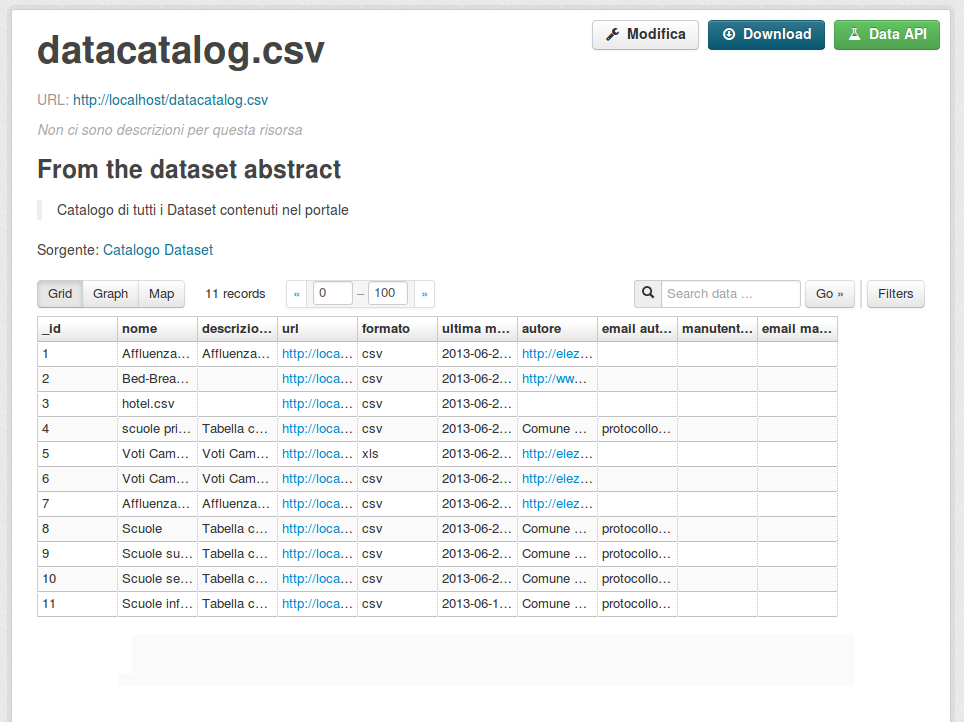
\includegraphics[scale=0.42]{img/demo-14-datacatalog}
   \caption{Catalogo dei dataset inseriti}
   \label{fig:demo-14-datacatalog}
\end{figure}

\newpage %nuova pagina

%-------------------------------------------------------------------------

\chapter{Conclusioni e sviluppi futuri}

%la tesi ha raggiunto i suoi obiettivi....
%sviluppi futuri
%integrazione a monte con git
%integrazione a valle con regione lombardia
%caricamento dataset

\newpage %nuova pagina

%-------------------------------------------------------------------------

\begin{thebibliography}{100}
\addcontentsline{toc}{chapter}{Riferimenti bibliografici}

%2.1
\bibitem{wiki-datiaperti}  Wikipedia - Dati aperti - 2013/06/29 - \url{https://it.wikipedia.org/wiki/Dati_aperti}
\bibitem{BernersLee-LinkedData} Tim Berners-Lee - LinkedData - 2009/06/18 - \url{http://www.w3.org/DesignIssues/LinkedData.html}
\bibitem{Direttiva-OpenGovernament} Peter R. Orszag - Open Government Directive - 2009/12/09 -\url{http://www.whitehouse.gov/sites/default/files/omb/assets/memoranda_2010/m10-06.pdf}
\bibitem{WhiteHouse-OpenData} The White House - Obama Administration Releases Historic Open Data Rules to Enhance Government Efficiency and Fuel Economic Growth - 2013/05/09 -\url{http://www.whitehouse.gov/the-press-office/2013/05/09/obama-administration-releases-historic-open-data-rules-enhance-governmen}
\bibitem{IODL2.0} Dati.gov.it - Italian Open Data License v2.0 - \url{http://www.dati.gov.it/iodl/2.0/}

%4.1
\bibitem{ComuneVigevano-CenniStorici} Comune di Vigevano - Cenni storici - \url{http://www.comune.vigevano.pv.it/territorio/cenni-storici}
\bibitem{ComuneVigevano-SIC} Comune di Vigevano - Servizio Informatico Comunale - SIC - \url{http://www.comune.vigevano.pv.it/canalitematici/servizio-informatico-comunale}

\end{thebibliography} 

%-------------------------------------------------------------------------
\end{document} %fine del documento